% $Id$

In chapter \ref{ch:inspiral} we saw that the gravitational waves from binary
inspiral take the form
\begin{equation}
h(t) = \mathcal{A} A(t) \cos\left( \phi(t) - \phi_0 \right)
\end{equation}
where $A(t)$ is the post$^{0}$-Newtonian amplitude, $\phi(t)$ is the
post$^2$-Newtonian phase evolution. The constants $\mathcal{A}$ and $\phi$ are
the unknown phase and amplitude of the waveform, respectively. In this chapter
we address the problem of finding such a signal hidden in detector noise. The
detection of signals of known form in noise is a well known
problem\cite{wainstein:1962}. In this chapter, we present the theory behind
such detection and then the particular implementation that we use to extract
inspiral signals from interferometer data in a computationally efficent manner.

\section{Dection of Gravitational Waves in Interferometer Noise}

The output of the interferometer, $s(t)$, may contain either random noise,
$n(t)$,
\begin{equation}
s(t) = n(t)
\end{equation}
or both the signal, $h(t)$, and random noise
\begin{equation}
s(t) = n(t) + h(t).
\end{equation}
Out goal is to decide if the signal is present or not. The interferometer
output always contains random noise so te test we use will be probabilistic in
nature. The test should give us the ``best'' answer to the question of signal
presence (we defer what we mean by best until later). We call this test the
\emph{optimum reciever} for the signal $h(t)$. The optimium reciever takes as
input the inteferometer data and returns as its output the consitional
probability, $P(h|s)$, that the signal, $h(t)$, is present given the data,
$s(t)$ and the conditional probability $P(0|s) = 1 - P(h|s)$ that the signal
is not present, given the data. The probabilities $P(h|s)$ and $P(0|s)$ are
\emph{a posteriori} probabilities. They are the result of an experiment to
determine if the signal is present in the data. The probability that the
signal is present before we conduct the experiment is the \emph{a priori}
probability $P(h)$. Similarly $P(0) = 1 - P(h)$ is the \emph{a priori}
probability that the signal is absent. To decide if the signal is present of
not, we construct a test on the output of the optimal reciever. Therefore we
need to know how to construct the optimal reciever and what decision rule to
apply to its output.

We begin with a review of some elementary probability.  The probability that
two events $A$ and $B$ occur simultaneously is given by
\begin{equation}
P(A,B) = P(A) P(B|A) = P(B) P(A|B).
\label{eq:probproduct}
\end{equation}
We may write equation (\ref{eq:probproduct}) in the form
\begin{equation}
P(A|B) = \frac{P(A,B)}{P(B)} = \frac{P(A)P(B|A)}{P(B)}
\label{eq:protobayes}
\end{equation}
If insted of a single event, $A$, suppose we have a complete set of mutually
exclusive events $A_1, A_2, \ldots, A_K$. By mutually exclusive we mean that
two or more of these events cannot occur simultaneously and by complete we
mean that one of them one of them must occur. Now suppose $B$ is an event that
can occur only if one of the $A_k$ occurs. Then the probability that $B$
occurs is given by
\begin{equation}
\begin{split}
P(B) &= P(A_1)P(B|A_1) + P(A_2)P(B|A_2) + \cdots + P(A_K)P(B|A_K) \\
     &= \sum_{k=1}^K P(A_k)P(B|A_k).
\end{split}
\label{eq:totalprob}
\end{equation}
Equation (\ref{eq:totalprob}) is called the \emph{total probability formula}.
Now let us suppose that $B$ is the result of an experiment and we want to know
the probability that it was event $A_k$ that allowed $B$ to happen. This can
be obtained by substituting equation (\ref{eq:totalprob}) into equation
(\ref{eq:protobayes}) to obtain
\begin{equation}
P(A_k|B) = \frac{P(A_k)P(B|A_k)}{P(B)} 
= \frac{P(A_k)P(B|A_k)}{\sum_{k=1}^K P(A_k)P(B|A_k)}.
\label{eq:bayeslaw}
\end{equation}
Equation (\ref{eq:bayeslaw}) is called \emph{Bayes' theorem}. The probability
$P(A_k)$ is the \emph{a priori} probability of event $A_k$ occuring and
$P(A_k|B)$ is the \emph{a posteriori} probability of $A_k$ occuring given
that the outcome of our experiment, $B$, occured. The conditional probability
$P(B|A_k)$ is called the \emph{likelihood}.

Now suppose that set $\{A_k\}$ contains only to two members: ``the signal is
present'' and ``the signal is absent''. The \emph{a priori} probabilities of
these events are $P(h)$ and $P(0)$, as discussed earlier. We consider $B$ to
be the output of the interferometer for a particular ``experiment''. Let us
Bayes' theorem to compute the \emph{a posteriori} probability that the signal
is present, given the ouput of the detector:
\begin{equation}
P(h|s) = \frac{P(h)P(s|h)}{P(s)}
\label{eq:pofhgivens1}
\end{equation}
where $P(s)$ is the \emph{a priori} probability of obtaining the detector
output and $P(s|h)$ is the likelihood function; the probability of obtaining
the detector output given that the signal is present in the data. The
probability of obtaining the detector output is given by
\begin{equation}
P(s) = P(h)P(s|h) + P(0)P(s|0)
\label{eq:pofs}
\end{equation}
and since the signal is either present or not, $P(h) + P(0) = 1$. Now we may
use equation (\ref{eq:pofs}) to write equation (\ref{eq:pofhgivens1}) as
\begin{equation}
P(h|s) = \frac{P(h)P(s|h)}{P(h)P(s|h) + P(0)P(s|0)}.
\label{eq:pofhgivens2}
\end{equation}
Dividing the numerator and denominator on the right hand side of equation
(\ref{eq:pofhgivens2}) by $P(h)P(s|0)$ we obtain
\begin{equation}
P(h|s) = \frac{P(s|h)/P(s|0)}{[P(s|h)/P(s|0)] + [P(0)P(h)]}.
\label{eq:pofhgivens3}
\end{equation}
Let us define the likelihood ratio, $\Lambda$, as
\begin{equation}
\Lambda = \frac{P(s|h)}{P(s|0)}
\label{eq:likelihooddef}
\end{equation}
and then equation (\ref{eq:pofhgivens3}) becomes
\begin{equation}
P(h|s) = \frac{\Lambda}{[\Lambda] + [P(0)P(h)]}.
\label{eq:pofhgivens4}
\end{equation}
Similarily, we find that the probability that the signal is absent is given by
\begin{equation}
P(0|s) = \frac{P(0)/P(h)}{\Lambda + [P(0)/P(h)}.
\label{eq:pofnothgivens}
\end{equation}
Using equations (\ref{eq:pofhgivens4}) and (\ref{eq:pofnothgivens}), we find
that the ratio of the \emph{a posteriori} probabilities that the signal is
present of absent, given the data is
\begin{equation}
\frac{P(h|s)}{P(0|s)} = \Lambda\frac{P(h)}{P(0)}.
\label{eq:postratio}
\end{equation}

We now construct an automated decision rule that will tell us if the signal is
present or absent.  If $P(h|s)$ is large (i.e.  close to unity) then it is
reasonable to conclude that the signal is present.  Conversely, if $P(h|s)$ is
small (close to zero) then we may conclude that the signal is absent.
Therefore we may set a threshold on this posterior probability, $P_\ast$, as
our decision rule is
\begin{equation}
\begin{split}
P(h|s) &\ge P_* \text{the signal is present}, \\
P(h|s) &< P_* \text{the signal is not present}.
\end{split}
\end{equation}
Given this decision rule there are four possible outcomes. If $P(h|s) \ge
P_*$ and the signal is present, we have made a correct detection. If $P(h|s)
\ge P_*$ and the signal is not present, we call this a \emph{false alarm}; our
decision that the signal is present was incorrect. If $P(h|s) < P_*$ and the
signal is not present, we have made a correct dismissal. Conversely, if
$P(h|s) < P_*$ and the signal is present, we have made a \emph{false
dismissal}. Each possible outcome has an accociated probability
\begin{align}
D & &&\text{probability that we make a correct detection} \\
F & &&\text{probability that we make a correct dismissal} \\
D' &= 1 - D &&\text{probability that we have a false alarm} \\
F' &= 1 - F &&\text{probability that we have a false dismissal}.
\end{align}
To construct the posterior probability, $P(h|s)$, and hence $P_\ast$, we need
the unknown \emph{a priori} probabilities, $P(h)$ and $P(0)$. We see from
equation (\ref{eq:pofhgivens4}), however, that $P(h|s)$ is a monotonically
increasing function of the likelihood. The ratio of the \emph{a priori}
probabilities, $P(h)/P(0)$, is a constant that does not invovle the result of
our experiment. Therefore we can define the output of out opitimum receiver to be
the device which, given the input data, $s(t)$ returns the likelihood ratio,
$\Lambda$, which does not involve the \emph{a priori} probabilities. 

For the reciever to be optimal in the Neyman-Pearson sense, we mean that for a
fixed false alarm probability, $F$, we maximize the detection probability,
$D$. It can be shown (see for example \cite{mathstat}) that the optimal
reciever is simply a threshold on the likelihood ratio:
\begin{equation}
\begin{split}
\Lambda &\ge \Lambda_\ast \text{the signal is present}, \\
\Lambda &< \Lambda_\ast \text{the signal is not present},
\end{split}
\end{equation}
where the threshold, $\Lambda_\ast$ is chosen based on the desired false alarm
probability, $F$. Thus, given the value of likelihood ratio, $\Lambda$, we
can then decide if the signal is present or absent. 

We now consider the construction of $\Lambda$ from the interferometer data,
$s(t)$ and the gravitational wave signal $h(t)$. Let us assume that the noise
is stationary and Gaussian with zero mean value
\begin{equation}
\left\langle n(t) \right\rangle = 0
\end{equation}
where angle brackets denote averaging over different ensembles of the
noise. The noise may be coloured, that is is contains correllations which are
expressed through its (one sided) power spectral density, $S_n(|f|)$, defined
by
\begin{equation}
\left\langle \tilde{n}(f) \tilde{n}(f') \right\rangle = \frac{1}{2} S_n(|f|)
\label{eq:ospsddef}
\end{equation}
where $\tilde{n}(f)$ is the Fourier transform of $n(t)$. We wish to compute
the quantity
\begin{equation}
\Lambda = \frac{P(s|h)}{P(s|0)} = 
\frac{p(s|h)\,ds}{p(s|0)\,ds} = \frac{p(s|h)}{p(s|0)}
\end{equation}
where $p(s|h)$ and $p(s|0)$ are the condition probability densities.  It can
be shown that if $n(t)$ is Gaussian noise, then the probability density of
obtaining a particular instant of noise is\cite{Finn:1992wt}
\begin{equation}
p(n) = \mathcal{K} \exp\left[-\frac{1}{2} (n|n)\right]
\end{equation}
where $\mathcal{K}$ is a normalization constant and the inner poduct
$(\cdot|\cdot)$ is given by
\begin{equation}
\label{eq:fullinnerproduct}
  (a\mid b) \equiv \int_{-\infty}^\infty df\,
  \frac{\tilde{a}^\ast(f)\tilde{b}(f)+\tilde{a}(f)\tilde{b}^\ast(f)}
       {S_n(|f|)}.
\end{equation}
The probability density of obtaining the interferometer output, $s(t)$, in the
absence of signal (i.e. $s(t) = n(t)$) is
\begin{equation}
p(s|0) = p(s) = \mathcal{K} \exp\left[-\frac{1}{2} (s|s)\right]
\end{equation}
The probability density of obtaining $s(t)$ in the presence of a signal (i.e.
when $s(t) = n(t) + h(t)$) is given by 
\begin{equation}
p(s|h) = p(s-h) = \mathcal{K} \exp\left[-\frac{1}{2} (s-h|s-h)\right]
\end{equation}
where we have used $n(t) = s(t) - h(t)$. Therefore the likelihood ratio
becomes
\begin{equation}
\begin{split}
\Lambda &= \frac{p(s|h)}{p(s|0)} = \frac{p(s-h)}{p(s)} \\
&= \frac{\exp\left[-\frac{1}{2} (s-h|s-h)\right]}{\exp\left[-\frac{1}{2} (s|s)\right]} \\
&= \exp\left\{-\frac{1}{2}\left[(s|s) - 2(s|h) - (h|h)\right] + \frac{1}{2}(s|s)\right\} \\
&= \exp\left[(s|h) - \frac{1}{2}(h|h)\right]
\end{split}
\end{equation}
where $(s|h)$ depends on the input data and $(h|h)$ is a constant (for a
given $S_n(|f|)$.) The likelihood ratio is therefore a monotonically
increasing function of $(s|h)$, so we insted of thresholding on $\Lambda$, we
can threshold on $(s|h)$. Our optimal reciver is now the construction of $(s|h)$
followed by a test
\begin{equation}
\begin{split}
(s|h) &\ge (s|h)_\ast \text{the signal is present}, \\
(s|h) &< (s|h)_\ast \text{the signal is not present},
\end{split}
\end{equation}
where the threshold is now $(s|h)_\ast$. For a given $h(t)$, the inner
product in equation $(\cdot|h)$, is a linear map from the infinite dimensional
vector space of signals to $\mathbb{R}$. Therefore the optimal reciever is a
linear function of the input signal, $s(t)$. For the data and signals that we
recieve are real functions of time, so 
\begin{align}
\tilde{s}^\ast(f) &= \tilde{s}(-f) \\
\tilde{h}^\ast(f) &= \tilde{h}(-f)
\end{align}
and the the inner product in equation (\ref{eq:fullinnerproduct}) becomes
\begin{equation}
\left(a\mid b\right) = 2 \int_{-\infty}^{\infty}df\,
\frac{\tilde{a}(f)\tilde{b}^\ast(f)}{S_n\left(\left|f\right|\right)}.
\label{eq:innerproduct}
\end{equation}

If we recieve only noise, then the mean of $(s|h)$ over a ensemble of detector
outputs is 
\begin{equation}
\begin{split}
\left\langle (s|h) \right\rangle &= \left\langle (n|h) \right\rangle \\
&= \int_{-\infty}^{\infty} 
   \frac{\langle\tilde{n}(f)\rangle \tilde{h}^\ast(f)}{S_n(|f|)} \\
&= 0
\end{split}
\end{equation}
since $\langle n(t) \rangle = 0$. The variance of $(s|h)$ in the absence of
signal is
\begin{equation}
\begin{split}
\left\langle(s|h)^2\right\rangle 
&= 2 \left\langle \int_{-\infty}^\infty \int_{-\infty}^\infty \,df\,df'\,
\frac{\tilde{n}(f)\tilde{h}^\ast(f) \tilde{n}^\ast(f')\tilde{h}(f')}
{S_n(|f|)\,S_n(|f'|)} \right\rangle \\
&= 2 \int_{-\infty}^\infty \int_{-\infty}^\infty \,df\,df'\,
\frac{\left\langle \tilde{n}(f)\tilde{n}^\ast(f')\right\rangle\tilde{h}^\ast(f)\tilde{h}(f')}
{S_n(|f|)\,S_n(|f'|)} \\
&= 2 \int_{-\infty}^\infty \int_{-\infty}^\infty \,df\,df'\,
\frac{\frac{1}{2}S_n(|f'|)\delta(f-f') \tilde{h}^\ast(f)\tilde{h}(f')}
{S_n(|f|)\,S_n(|f'|)} \\
&= (h|h)
\end{split}
\end{equation}
where we have used equation (\ref{eq:ospsddef}).  In the presence of signal
and noise, then the mean of $(s|h)$ is
\begin{equation}
\left\langle (n+h|h) \right\rangle = (\rangle n \langle + h|h) = (h|h).
\end{equation}
We can also show that the variance of $(s|h)$ in the presence of signal is
\begin{equation}
\left\langle (s|h)^2 \right\rangle 
= \left\langle \left[ (s|h) - (h|h) \right]^2 \right\rangle
= \left\langle \left[ (n|h) \right]^2 \right\rangle
= (h|h).
\end{equation}
Therefore the quantity $(h|h)$ is the variance of the output of the optimal
reciever, $(s|h)$, and we denote it by
\begin{equation}
\sigma^2 \equiv (h|h).
\end{equation}

Now suppose that the signal we wish to recover has an unknown amplitude,
$\mathcal{A}$. The above discussion holds with $h(t) \rightarrow
\mathcal{A}h(t)$ and the likelihood ratio becomes
\begin{equation}
\Lambda = \exp\left[\mathcal{A}(s|h) - \frac{1}{2}\mathcal{A}^2(h|h)\right]
\end{equation}
which is monotonic in $(s|h)$, and so our previous choise of optimal statistic
an threshold holds. Now we are ready to consider the case of a true
gravitational wave signal, which has unknown amplitude, $\mathcal{A}$, and
unknown phase, $\theta$:
\begin{equation}
h(t) = \mathcal{A} A(t) \cos(\phi(t) - \theta).
\end{equation}
The likelihood ratio now becomes a function of $\theta$
\begin{equation}
\Lambda'(\theta) = 
p(\theta|h) \exp\left[\mathcal{A}(s|A(t)\cos(\phi(t) - \theta) -
\frac{1}{2}\mathcal{A}^2(h|h)\right].
\end{equation}
Now consider the first inner product in the above exponential. Using
$\cos(\phi - \theta) = \cos\theta\cos\phi + \sin\theta\sin\phi$ we may write
this as
\begin{equation}
\begin{split}
(s|A(t)\cos(\phi(t) - \theta)  &= 
\cos\theta (s|A(t)\cos(\phi(t))) + \sin\theta (s|A(t)\sin(\phi(t)))  \\
& = x\cos\theta + y\cos\theta \\
& = z\cos(\Phi - \theta)
\end{split}
\end{equation}
where
\begin{align}
x &= z\cos\Phi = (s|A(t)\cos(\phi(t))), \\
y &= z\sin\Phi = (s|A(t)\sin(\phi(t))), \\
z &= \sqrt{x^2 + y^2}, \\
\tan \Phi &= \frac{y}{x}.
\end{align}
To calculate the likelihood ratio, $\Lambda$, we assume that the unknown phase
is uniformly distributed between $0$ and $2\pi$,
\begin{equation}
p(\theta|h) = \frac{1}{2\pi},
\end{equation}
and integrate $\Lambda'$ over the angle $\theta$. We obtain
\begin{equation}
\begin{split}
\Lambda &= \int_0^{2\pi} \Lambda'(\theta) 
= \frac{1}{2\pi}\int_0^{2\pi}\exp\left[\mathcal{A}z\cos(\Phi - \theta) -
\mathcal{A}^2)(h|h)\right] \,d\theta \\
&= I_0(Az) e^{-\mathcal{A}^2\frac{1}{2}(h|h)}
\end{split}
\end{equation}
where $I_0$ is the modified Bessel function of the first kind of order zero.
The function $I_0(Az)$ is a monotonically increasing function of $z$ and so we
can threshold on $z$ insted of $\Lambda$. Therefore to construct an optimal
reciever for a signal of unknown amplitude and phase, we can threshold on $z$.

To compute the optimal reciever for a binary inspiral signal, we compute the
two inner products $x = (s|A(t)\cos\phi(t))$ and $y = (s|A(t)\sin\phi(t))$. We
then threshold on $z = \sqrt{x^2+y^2}$ with a threshold $z_\ast$, set by our
desired false alarm rate, and then our detection decision is
\begin{equation}
\begin{split}
z &\ge z_* \text{the signal is present}, \\
z(h|s) &< z_* \text{the signal is not present}.
\end{split}
\end{equation}
Recall from chapter \ref{ch:inspiral} that we denoted the two orthogonal
phases of the binary inspiral waveform by $h_c$ and $h_s$ and
\begin{align}
h_c(t) &\propto f^\frac{2}{3}(t) \cos(\phi(t)) \\
h_s(t) &\propto f^\frac{2}{3}(t) \sin(\phi(t)) \\
\end{align}
so the construction of $z$ becomes
\begin{equation}
z = \sqrt{(s|h_c)^2 + (s|h_s)^2}.
\end{equation}
The inspiral waveforms are orthogonal, so $(h_c|h_s) = 0$. We can also see
that $(h|h) = (h_c|h_c) = (h_s|h_s)$. Notice that the inner product,
$(\cdot|\cdot)$ contains the power spectral density, $S_n(f)$. This means that
if $S_n(f)$ changes, we must change the threshold $z_\ast$. To remove this
dependence, we construct the \emph{signal-to-noise ratio}, $\rho$, defined by
\begin{equation}
\rho = \frac{z}{\sqrt{(h_c|h_c)}} = \frac{z}{\sigma}
\end{equation}
and threshold on $\rho \ge \rho_\ast$.

If a gravitational wave signal is present, then its location in time is
defined by the \emph{end time} of the waveform, $t_e$. In chapter
\ref{ch:inspiral} we defined the end time of the chirp to be the time at which
the frequency of the gravitational wave reached $f_\mathrm{isco}$, the
gravitational wave frequency of a particle in the innermost stable circular
orbit of Scharzschild spacetime.  In the above discussion of the optimal
reciever, we implicitly knew the location of the signal in the data, say 
$t_e = 0$. Now suppose that the inspiral waveform ends at some unknown time,
$t_e = t$. We may write the signal we are searching for as $h(t'-t)$. Consider
the Fourier transform of this signal
\begin{equation}
\begin{split}
\int_{-\infty}^\infty e^{-2\pi i f t'} h(t'-t) \, dt' &= 
e^{-2\pi ift} \int_{-\infty}^\infty e^{-2\pi i f \tau} h(\tau) \, d\tau \\
&= e^{-2\pi ift} \tilde{h}(f).
\end{split}
\end{equation}
where we have used $\tau = t' - t$, $dt = d\tau$ and $t' = t + \tau$.
The value of the inner product $(s|h_c)$ for a waveform that ends at time $t$ is
therefore
\begin{equation}
(s|h_c(t)) = 2 \int_{-\infty}^\infty\,df e^{2\pi ift}
\frac{\tilde{s}(f)\tilde{h}^\ast(f)}{S_n(|f|)}
\label{eq:ipift}
\end{equation}
and the signal-to-noise ratio for a chirp that ends at time $t$ is
\begin{equation}
\rho(t) = \frac{1}{\sigma} \sqrt{ (s|h_c(t))^2 + (s|h_s(t))^2}
\end{equation}
where the quantities $(s|h_c(t))$ and $(s|h_s(t))$ can be obtained by inverse
Fourier transforms. This is of particular importance as we can compute the
entire signal-to-noise ratio for a segment of digitally sampled data using the
Fast Fourier Transform, as we will see below. We have now completely specified
the solution to the problem of finding a waveform of unknown amplitude and
phase at an unknown position in the data; our optimim reciever is the
\emph{matched filter}. In the sections below we develop the techniques that we
use to construct a digital implementation of the matched filter to search for
gravitational wave signals in interferometer data.

\section{Conventions}
\label{s:conventions}

The raw (uncalibrated) output of the detector is a time series denoted $v(t)$.
In practice, this is discretely sampled data with sampling interval $\Delta
t$, that is $v_j \equiv v(t_j)$ where $t_j = j\Delta t$.  In order to
construct a digital matched filter, we take $N$ consecutive samples of
$v(t_j)$. We will always follow the convention that the subscript $j$ refers to
discretely sampled time domain quantities and the subscript $k$ to discretely
sampled frequency domain quantities. Other subscripts, such as $i$, refer to
iteration over other quantities such as inspiral template index. For a
frequency domain quantity $\tilde{v}(f_k)$ denotes the value quantity samples
at a particular frequency $f_k$ whereas $\tilde{v}_k = \tilde{v}(f_k) / \Delta
t$ denotes the same quantity divided by the sampling interval.

\subsection{The Fourier Transform}
\label{ss:ftconv}

We define the forward Fourier transform $\tilde{v}(f)$ of a time domain
quantity $v(t)$ to be
\begin{equation}
\label{eq:ft}
\tilde{v}(f)=\int_{-\infty}^\infty dt\,v(t)\, e^{- 2 \pi i f t}
\end{equation}
and the inverse Fourier transform to be 
\begin{equation}
\label{eq:ift}
v(t)=\int_{-\infty}^\infty df\,\tilde{v}(f)\, e^{2 \pi i f t}.
\end{equation}

For the $N$ sample points $v_j$ we may estimate the Fourier transform at 
$N + 1$ samples in the range $[-f_n,f_n]$, where $f_n = 1/(2\Delta t)$ is the
Nyquist critical frequency, by
\begin{equation}
\tilde{v}(f_k) \approx \sum_{j=0}^{N-1} \Delta t\, h(t_j) e^{-2 \pi i f_k t_j}
= \Delta t \sum_{j=0}^{N-1} v_j e^{-2 \pi i j k / N}.
\end{equation}
There are only $N$ independent values of $\tilde{v}(f_k)$ as the extreme
values of $k$ correspond to the upper and lower limits of the Nyquist
frequency range and are equal. The discrete Fourier transform is the defined
to be\cite{T010095}
\begin{equation}
\tilde{v}_k = \sum_{j=0}^{N-1} v_j e^{-i 2 \pi j k / N}.
\end{equation}
We may estimate the discrete inverse Fourier transform from equation
(\ref{eq:ift}) using
\begin{equation}
\Delta f = f_{k+1} - f_k = \frac{k+1}{N\Delta t} - \frac{k}{N\Delta t} =
\frac{1}{N\Delta t}
\end{equation}
which gives
\begin{equation}
v(t_j) \approx \sum_{k=0}^{N-1} \tilde{v}(f_k) e^{2 \pi i f_k t_j / N} \Delta f
= \frac{1}{N} \sum_{k=0}^{N-1} \tilde{v}_k e^{2 \pi i j k / N}.
\end{equation}

\subsection{Power Spectral Densities}
\label{ss:psdconv}

Consider a signal $n(t)$ containing Gaussian noise and dimensions $U$, which
may be voltage, strain, etc. We define the one sided power spectral density,
$\ospsd$, of this signal by the equation
\begin{equation}
\left\langle\tilde{n}(f) \tilde{n}^\ast(f')\right\rangle = 
\frac{1}{2}\ospsd\delta(f-f)
\end{equation}
which has units of $\mathrm{time}\times U^2$. For discretely sampled 
quantities we have
\begin{equation}
\left\langle\tilde{n}(f_k) \tilde{n}^\ast(f_{k'})\right\rangle = 
\frac{1}{2}\ospsd\delta(f_k-f_{k'})
\end{equation}
which gives
\begin{equation}
\label{eq:psddef}
\left\langle\tilde{n}_k \tilde{n}_{k'}^\ast\right\rangle = 
\frac{N}{2\Delta t}\ospsd\delta_{kk'}
\end{equation}
which defines \ospsd in terms of the discrete frequency domain quantities.
The definition in equation (\ref{eq:psddef}) is equivalent to
\begin{equation}
\ospsd = \left\{
\begin{array}{ll}
\frac{\Delta t}{N} | \tilde{n}_0 |^2 & k = 0, \\
\\
\frac{\Delta t}{N} \left[ | \tilde{n}_k |^2 + | \tilde{n}_{N-k} |^2 \right] &
k\neq 0.
\end{array}
\right.
\end{equation}

\section{Matched Filtering}
\label{s:matchedfilter}

The dimensionless strain $h(t)$ of the gravitational wave produces a
differential change $\Delta L(t)=L h(t)$ in the lengths of the two
perpendicular interferometer arms, where $L$ is the average arm length.  In
addition the gravitational wave signal that we wish to detect the
interferometer output contains noise, $n(t)$. We assume that the noise samples
are drawn from a stationary Gaussian distribution, though there may be
correlations among the noise events (colored noise). The noise correlations
may be expressed in terms of the one-sided noise power spectral density,
\ospsd, defined in equation (\ref{eq:psddef}). The (calibrated) detector
output is $s(t) = h(t) + n(t)$.  Our problem is to detect the presence of a
gravitational wave signal $h(t)$ in the detector output $s(t)$.

\subsection{The maximum likelihood receiver}
\label{ss:maxrec}

A comprehensive discussion of the statistical theory of signal detection can
be found in~\cite{wz} and in the context of binary inspiral
in~\cite{finn,finnchernoff}. The reception process is simply the construction
of some statistic of the data followed by a test of the hypotheses ``there is
a signal present in the data'' and ``there is no signal present in the data.''
When these hypothesis are assumed to be mutually exclusive, the reception
process reduces to the comparison of the statistic with some pre-assigned
threshold. 

As described in section \ref{s:waveforms}, the gravitation radiation from a
binary inspiral is a linear combination of two possible orbital phases,
$h_{+}$ and $h_{\times}$ at a physical distance $\mathcal{D}$. This means that
the signal that we wish to detect, $h(t)$, is known up to an arbitrary phase
$\theta$ and amplitude $A$,
\begin{equation}
h(t) = A \cos \theta h_c(t) + A \sin \theta h_s(t)
\end{equation}
Here we review the construction of a statistic which is optimal for
signals which are known up to an arrival time and phase which are to be
determined.

\textcolor{red}{Add section on statistical theory of matched filtering from
thesis.} We define an inner product $(\cdot|\cdot)$ by
\begin{equation}
\label{eq:innerproduct}
  (a\mid b) \equiv \int_{-\infty}^\infty df\,
  \frac{\tilde{a}^\ast(f)\tilde{b}(f)+\tilde{a}(f)\tilde{b}^\ast(f)}
       {S_n(|f|)}.
\end{equation}
Since the chirp waveforms are are real time series, we have $h(f) =
h^\ast(-f)$ and the inner product (\ref{eq:innerproduct}) becomes
\begin{equation}
\left(a\mid b\right) = 2 \int_{-\infty}^{\infty}df\,
\frac{\tilde{a}^\ast(f)\tilde{b}(f)}{S_n\left(\left|f\right|\right)}.
\label{eq:innerproduct2}
\end{equation}

The sine and cosine polarizations of the inspiral signal are orthogonal,
\begin{equation}
\left(h_c\mid h_s\right) = 0.
\end{equation}
We define the normalization constant $\sigma^2$ to be
\begin{equation}
\sigma^2 \equiv \left(h_c\mid h_c\right) = \left(h_s\mid h_s\right).
\label{eq:sigmasqdef}
\end{equation}

The inspiral signals that we wish to receive are much shorter than the
observation time, and we do not know when the signals occur. We wish not only
to detect these signals, but also to measure their arrival time. To do so, we
construct the time series
\begin{equation}
\label{eq:xcts}
x(t) = 2 \int_{-\infty}^{\infty}df\,e^{2\pi i f t} 
\frac{\tilde{s}(f) \tilde{h_c}^\ast(f)}{S_n\left(\left|f\right|\right)}
\end{equation}
and
\begin{equation}
\label{eq:ycts}
y(t) = 2 \int_{-\infty}^{\infty}df\,e^{2\pi i f t} 
\frac{\tilde{s}(f) \tilde{h_s}^\ast(f)}{S_n\left(\left|f\right|\right)}.
\end{equation}
For each observation period, we construct the statistic
\begin{equation}
\rho(t) = \frac{1}{\sigma}\sqrt{x^2(t) + y^2(t)}
\label{eq:rhosqcts}
\end{equation}
and threshold on this statistic, which we call the signal-to-noise ratio
(SNR). From equation (\ref{eq:sigmasqdef}) the normalization constant $\sigma$ is
\begin{equation}
\label{eq:sigmasqcts}
\sigma^2 = 2 \int_{-\infty}^{\infty}df\,
\frac{\tilde{h_c}^\ast(f)\tilde{h_c}(f)}{S_h\left(\left|f\right|\right)} 
= 2 \int_{-\infty}^\infty 
\frac{\tilde{h_s}^\ast(f)\tilde{h_s}(f)}{S_h\left(\left|f\right|\right)}.
\end{equation}
The filter that we have constructed is normalized according to the convention
of Cutler and Flanagan \cite{cutflan}, so that in the case when the detector
output is Gaussian noise, the filter output averaged over an ensemble of
detectors with different realizations of the noise is
$\left\langle \rho^2 \right\rangle = \left\langle x^2 + y^2 \right\rangle = 2$.

\subsection{Construction of the digital filter using stationary phase chirps}
\label{ss:digitalfilter}

Since the two chirp waveforms $\tilde{h_c}$ and $\tilde{h_s}$ are 
orthogonal, it is possible to increase the efficiency of the algorithm by
constructing the time series $\rho(t)$ directly using a single complex inverse
FFT rather than computing it from $x(t)$ and $y(t)$ which requires two real
inverse FFTs. We may further increase efficiency when using stationary phase
chirps by dividing the filter into a part that depends on the data and a part
that depends only on the template parameters. In this section we describe the
construction of a digital matched filter which uses these two methods.
Consider the discrete form of equation (\ref{eq:xcts})
\begin{equation}
\begin{split}
\label{eq:xdisc}
x_j &= \frac{2}{\sigma} \frac{1}{N\Delta t} \sum_{k=0}^{N-1} e^{2\pi ijk/N} 
\frac{\tilde{s}(f_k) \tilde{h}_{c}^\ast(f_k)}{\ospsd} \\
&=
\frac{2}{\sigma} \frac{\Delta t}{N} \sum_{k=0}^{N-1} e^{2\pi ijk/N} 
\frac{\tilde{s}_k \tilde{h}_{ck}^\ast} {\ospsd}
\end{split}
\end{equation}
where we have used $\tilde{s}(f_k) = \Delta t\, \tilde{s}_k$ and
${h}_c(f_k) \equiv \Delta t\, \tilde{h}_{ck}$. From equation
(\ref{eq:ycts}) we obtain
\begin{equation}
\label{eq:ydisc}
y_j = \frac{2}{\sigma} \frac{\Delta t}{N} \sum_{k=0}^{N-1} e^{2\pi ijk/N} 
\frac{\tilde{s}_k \tilde{h}_{sk}^\ast} {\ospsd}
\end{equation}
The normalization constant $\sigma^2$ defined in equation
(\ref{eq:sigmasqcts}) is
\begin{equation}
\begin{split}
\label{eq:sigmasqdisc}
\sigma^2 &= 2 \frac{1}{N\Delta t} \sum_{k=0}^{N-1}
\frac{\tilde{h}_{c}(f_k)\tilde{h}_{c}^\ast(f_k)}{\ospsd}  \\
&=
2 \frac{\Delta t}{N} \sum_{k=0}^{N-1}
\frac{\tilde{h}_{ck}\tilde{h}_{ck}^\ast}{\ospsd} \\
&=
4 \frac{\Delta t}{N} \sum_{k=0}^{N/2}
\frac{\tilde{h}_{ck}\tilde{h}_{ck}^\ast}{\ospsd}.
\end{split}
\end{equation}
Now we may use the fact that $s(t)$ is a real signal and so $\tilde{s}(f) = 
\tilde{s}(-f)^\ast$ to write equation the cosine phase of the filter 
(\ref{eq:xdisc}) as
\begin{equation}
\begin{split}
x_j &= 
\frac{2}{\sigma}\frac{\Delta t}{N}
\left[
  \sum_{k=N/2}^{N-1} e^{2\pi ijk/N} 
  \frac{\tilde{s}_k \tilde{h}_{ck}^\ast}{\ospsd}
  +
  \sum_{k=0}^{N/2} e^{2\pi ijk/N} 
  \frac{\tilde{s}_k \tilde{h}_{ck}^\ast}{\ospsd}
\right] \\
&= \frac{2}{\sigma}\frac{\Delta t}{N}
\left[
  \sum_{k=0}^{N/2} e^{-2\pi ijk/N} 
  \frac{\tilde{s}_k^\ast \tilde{h}_{ck}}{\ospsd}
  +
  \sum_{k=0}^{N/2} e^{2\pi ijk/N} 
  \frac{\tilde{s}_k \tilde{h}_{ck}^\ast}{\ospsd}
\right] \\
&= \frac{2}{\sigma}\frac{\Delta t}{N}(Q_j^\ast + Q_j)
\end{split}
\end{equation}
where
\begin{equation}
\label{eq:Qdef}
Q_j = \sum_{k=0}^{N/2} e^{2\pi ijk/N} 
  \frac{\tilde{s}_k \tilde{h}_{ck}^\ast}{\ospsd}.
\end{equation}
The sine phase of the filter (\ref{eq:ydisc}) can be written as
\begin{equation}
\begin{split}
\label{eq:yinter}
y_j &=
\frac{2}{\sigma}\frac{\Delta t}{N}
\left[
  \sum_{k=N/2}^{N-1} e^{2\pi ijk/N} 
  \frac{\tilde{s}_k \tilde{h}_{sk}^\ast}{\ospsd}
  +
  \sum_{k=0}^{N/2} e^{2\pi ijk/N} 
  \frac{\tilde{s}_k \tilde{h}_{sk}^\ast}{\ospsd}
\right] \\
&= 
\frac{2}{\sigma}\frac{\Delta t}{N}
\left[
  \sum_{k=0}^{N/2} e^{-2\pi ijk/N} 
  \frac{\tilde{s}_k^\ast \tilde{h}_{sk}}{\ospsd}
  +
  \sum_{k=0}^{N/2} e^{2\pi ijk/N} 
  \frac{\tilde{s}_k \tilde{h}_{sk}^\ast}{\ospsd}
\right]
\end{split}
\end{equation}
Using (\ref{eq:hsorthog}), equation (\ref{eq:yinter}) becomes
\begin{equation}
\begin{split}
y_j &= 
\frac{2}{\sigma}\frac{\Delta t}{N}
\left[
  \sum_{k=0}^{N/2} e^{-2\pi ijk/N} 
  \frac{\tilde{s}_k^\ast i\tilde{h}_{ck}}{\ospsd}
  +
  \sum_{k=0}^{N/2} e^{2\pi ijk/N} 
  \frac{\tilde{s}_k (-i)\tilde{h}_{ck}^\ast}{\ospsd}
\right] \\
& = 
\frac{-2i}{\sigma}\frac{\Delta t}{N}
\left[
  - \sum_{k=0}^{N/2} e^{-2\pi ijk/N} 
  \frac{\tilde{s}_k^\ast \tilde{h}_{ck}}{\ospsd}
  +
  \sum_{k=0}^{N/2} e^{2\pi ijk/N} 
  \frac{\tilde{s}_k \tilde{h}_{ck}^\ast}{\ospsd}
\right] \\
& = 
\frac{2}{\sigma}\frac{\Delta t}{N}i(Q_j^\ast - Q_j).
\end{split}
\end{equation}
Thus the outputs of the filter for the two phases are
\begin{equation}
x_j = \frac{4}{\sigma} \Re z_j,
\quad\mathrm{and}\quad
y_j = \frac{4}{\sigma} \Im z_j.
\end{equation}
The quantity $z_j$ is defined to be
\begin{equation}
\begin{split}
\label{eq:zdef}
z_j &= \frac{\Delta t}{N}\sum_{k=0}^{N/2} e^{2\pi ijk/N} 
\frac{\tilde{s}_k \tilde{h}_{ck}^\ast}{\ospsd}  \\
&= \frac{\Delta t}{N}\sum_{k=0}^{N-1} e^{2\pi ijk/N} \tilde{z}_k
\end{split}
\end{equation}
where
\begin{equation}
\label{eq:ztildedef}
\tilde{z}_k = \left\{
\begin{array}{ll}
\frac{\tilde{s}_k \tilde{h}_{ck}^\ast}{\ospsd} 
  \quad\quad & 0 < k < \frac{N}{2},\\
\\
0 & \mathrm{otherwise}.
\end{array}
\right.
\end{equation}
We can now compute the square of the signal-to-noise ratio
\begin{equation}
\rho^2(t_j) = x_j^2 + y_j^2 = \frac{16}{\sigma^2}|z_j|^2
\end{equation}
by a single complex inverse Fourier transform and threshold on 
$\rho^2 \ge \rho^2_\ast$.  Since we choose the 2~PN stationary phase template
chirp $\tilde{h}_c(f)$ to be at a canonical distance of $1$~Mpc, the effective
distance $\mathcal{D}$ to a chirp detected with signal to noise ratio $\rho^2$
is then given by
\begin{equation}
\mathcal{D}\,(\mathrm{Mpc})= \sqrt{\frac{\sigma^2}{\rho^2}}.
\end{equation}

The calibrated detector output is related to the raw detector output by the
detector response function according to
\begin{equation}
\tilde{s}(f) = R(f;t) \tilde{v}(f)
\end{equation}
where $R(f;t)$ is the (complex) response function of the detector at a
specific time $t$\cite{calpaper}. In practice, we compute the uncalibrated
power spectral density $S_v(|f_k|)$ from the raw data and then the calibrated
power spectral density, $\ospsd$, in the denominator of (\ref{eq:zdef}) is
\begin{equation}
\ospsd = |R(f;t)|^2 S_v(|f_k|).
\end{equation}
Further details of the computation of $S_v(|f_k|)$ are given in sections
\ref{ss:psd} and \ref{ss:invspec}.

Typical values of the variance of $v(t)$ for initial LIGO data are $10^3$,
however the response function, $R(f)$, has magnitude $\sim 10^{-22}$ in the
sensitive band of the instrument. Although we only need floating point (4
byte) precision to store the calibrated interferometer data, $\tilde{s}(f)$
and the power spectral density, $S_n(|f|)$, the calibrated time domain data may
overflow the dynamic range of floating point variables. Therefore when we
implement the digital filter, we multiply the response function $R(f)$ by a
scaling variable, $d$, which typically has values of $d = 2^{64}$ for initial
LIGO data. This scales all frequency domain quantities to of order  
unity.  Therefore equation (\ref{eq:zdef}) becomes
\begin{equation}
\label{eq:zdefcal}
z_j = \sum_{k=0}^{N/2} e^{2\pi ijk/N} 
  \frac{dR\tilde{v}_k\, d\tilde{h}_{ck}^\ast}
  {d^2|R|^2S_v\left(\left|f_k\right|\right)}
\end{equation}
and (\ref{eq:sigmasqdisc}) becomes
\begin{equation}
\label{eq:sigmasqdisccal}
\sigma^2 = 4 \frac{\Delta t}{N} \sum_{k=0}^{N/2}
\frac{d^2 \tilde{h}_{ck}\tilde{h}_{ck}^\ast}
{d^2|R|^2S_v\left(\left|f_k\right|\right)}. 
\end{equation}
Notice that we must also multiply the chirp by $d$ so that all the factors of
$d$ cancel in the signal-to-noise ratio, $\rho(t_j)$, and the normalization
constant, $\sigma^2$. In fact this is convenient as it brings the value of
the strain $h_c(f_k)$ to order unity. From equation (\ref{eq:spcos}) we obtain
the (dimensionless) quantity
\begin{equation}
\begin{split}
\label{eq:hck}
d\,\tilde{h}_{ck} &= \frac{d \tilde{h}_c(f_k)}{\Delta t} \\
&= 
\frac{2dT_\odot c}{1\,\mathrm{Mpc}}
\left(\frac{5\mu}{96M_\odot}\right)^\frac{1}{2}
\left(\frac{M}{\pi^2M_\odot}\right)^\frac{1}{3}
\left(\frac{T_\odot}{\Delta t}\right)^{-\frac{1}{6}}
\left( f\,\Delta t \right)^{-\frac{7}{6}}
\exp\,[i\Psi(f_k;M,\eta)] \theta\left(k-k_\mathrm{ISCO}\right)\\
&=
\sqrt{\mathcal{T}(M,\mu)}\left(\frac{k}{N}\right)^{-\frac{7}{6}}
\exp\left[i\Psi\left(f_k;M,\eta\right)\right] \theta\left(k-k_\mathrm{ISCO}\right)
\end{split}
\end{equation}
where the term $\theta\left(k-k_\mathrm{ISCO}\right)$ ensure that the chirp is
terminated at $k = k_\mathrm{ISCO} = f_\mathrm{ISCO} / \Delta f$ and we have 
defined the quantity $\mathcal{T}(M,\mu)$ to be
\begin{equation}
\mathcal{T}(M,\mu) = \left[
\left(\frac{2dT_\odot c}{1\,\mathrm{Mpc}}\right)
\left(\frac{5\mu}{96M_\odot}\right)^\frac{1}{2}
\left(\frac{M}{\pi^2M_\odot}\right)^\frac{1}{3}
\left(\frac{T_\odot}{\Delta t}\right)^{-\frac{1}{6}}
\right]^2.
\end{equation}
$\mathcal{T}$ is referred to as the \emph{template dependent normalization
constant}. It depends on the masses of the template and as such must be
recomputed once per template. If we substitute equation (\ref{eq:hck}) 
into equation (\ref{eq:sigmasqdisccal}) we obtain
\begin{equation}
\sigma^2 = 4 \frac{\Delta t}{N} \mathcal{T} 
\sum_{k=0}^{k_\mathrm{ISCO}} 
\frac{\left(\frac{k}{N}\right)^{-\frac{7}{3}}}
{d^2|R|^2S_v\left(\left|f_k\right|\right)}
= 4 \frac{\Delta t}{N} \mathcal{T} \mathcal{S}
\end{equation}
where $\mathcal{S}$ is defined to be
\begin{equation}
\mathcal{S} = 
\sum_{k=0}^{k_\mathrm{ISCO}} 
\frac{\left(\frac{k}{N}\right)^{-\frac{7}{3}}}{d^2|R|^2S_v\left(\left|f_k\right|\right)}.
\end{equation}
$\mathcal{S}$ is referred to as the \emph{segment dependent normalization}.
We compute and store the array 
\begin{equation}
\mathcal{S}(k_\mathrm{ISCO}) \quad \quad 0 < k_\mathrm{ISCO} < \frac{N}{2}
\end{equation}
from the input power spectral density. We then select the correct value of
$\mathcal{S}$ for each chirp my computing the $f_\mathrm{ISCO}$ of the
template.

The signal-to-noise ratio squared is then
\begin{equation}
\rho^2(t_j) = 
\frac{16}{\sigma^2}\left(\frac{\Delta t}{N}\right)^2 \mathcal{T}
\left| 
  \sum_{k=0}^{N/2} e^{2\pi ijk/N} 
  \frac{dR\tilde{v}_k \left(\frac{k}{N}\right)^{-\frac{7}{6}} \exp\left[-i\Psi(f_k;M,\eta)\right] \theta\left(k-k_\mathrm{ISCO}\right)}
       {d^2|R|^2 S_v\left(\left|f_k\right|\right)}
\right|^2 
\label{eq:signaltonoisesq}
\end{equation}
where $\sigma^2$ is simply
\begin{equation}
\sigma^2 = \frac{4\Delta t}{N} \mathcal{T}\mathcal{S}.
\label{eq:sigmasqts}
\end{equation}
Let us define $\tilde{q}_k$ by
\begin{equation}
\label{eq:qtildedef}
\tilde{q}_k = \left\{
\begin{array}{ll}
\frac{d\tilde{v}_k \left(\frac{k}{N}\right)^{-\frac{7}{6}} \exp\left[-i\Psi(f_k;M,\eta)\right]}
     {d^2|R|^2S_v\left(\left|f_k\right|\right)} 
  \quad\quad & 0 < k < k_\mathrm{ISCO},\\
\\
0 & \mathrm{otherwise}.
\end{array}
\right.
\end{equation}
and $q_j$ as the discrete inverse Fourier transform of $\tilde{q}_k$, then
the signal-to-noise ratio squared is
\begin{equation}
\rho^2(t_j) = \frac{16}{\sigma^2}\left(\frac{\Delta T}{N}\right)^2 \mathcal{T}
\left|q_j\right|^2
\end{equation}
The computation of $\tilde{q}_k$ can further be split into the template
independent computation of
\begin{equation}
\tilde{F}_k = \frac{d\tilde{v}_k \left(\frac{k}{N}\right)^{-\frac{7}{6}}}
{d^2|R|^2S_v\left(\left|f_k\right|\right)}
\end{equation}
and the computation of
\begin{equation}
\tilde{T}_k = \exp\left[i\Psi(f_k;M,\eta)\right] \theta\left(k-k_\mathrm{ISCO}\right)
\end{equation}
where $\tilde{F}_k$ is called the \emph{findchirp data segment} and 
$\tilde{T}_k$ is called the \emph{findchirp template}, so
\begin{equation}
\tilde{q}_k = \left\{
\begin{array}{ll}
\tilde{F}_k \tilde{T}_k^\ast \quad\quad & 0 < k < \frac{N}{2},\\
\\
0 & \mathrm{otherwise}.
\end{array}
\right.
\end{equation}

In practice we construct the average power spectral density from $M$ data
segments and then this $\ospsd$ to filter each of the $M$ segments for
inspiral signals. Using the above relationships, we only need to compute
$\mathcal{S}(k_\mathrm{ISCO})$ once per PSD and $\tilde{F}_k$ once per data
segment. We can then store these quantities re-use them, computing
$\mathcal{T}$ and $\tilde{T}_k$ once per template. We also save some
computational effort by computing
\begin{equation}
|q|^2_\ast = \frac{\rho^2_\ast} 
{\frac{16}{\sigma^2}\left(\frac{\Delta t}{N}\right)^2 \mathcal{T}}
\end{equation}
and thresholding on $|q_j|^2 \ge |q|^2_\ast$. We describe the algorithm used to
generate the inspiral triggers in section \ref{s:maxoverchirp} below.

\section{Testing the filtering code}
\label{s:testing}

\subsection{Normalization}
\label{ss:normalization}

In section \ref{s:maxrec} we showed that we can construct a quantity $\rho^2$
and threshold on this to decide if a signal is present in the data. In section
\ref{ss:digitalfilter} we described how the construction of $\rho^2$ is
implemented in the digital filtering code. In this section, we consider some 
testing of the most basic tests of the inspiral filtering code.

Consider the case when the filter input is Gaussian noise, i.e. $\tilde{s}_k =
\tilde{n}_k$.  We will also set $R(f_k)\equiv 1$ and $d = 1$.  Then the expectation
value of the signal-to-noise ratio squared, $\langle \rho^2
\rangle$ is
\begin{equation}
\begin{split}
\langle \rho^2(t_j) \rangle &=
\frac{16}{\sigma^2}\left(\frac{\Delta t}{N}\right)^2 \mathcal{T}
  \sum_{k=0}^{N/2} \sum_{k'=0}^{N/2} 
  e^{2\pi ij(k-k')/N} 
  \frac{\left\langle \tilde{n}_k \tilde{n}_{k'}^{\ast} \right\rangle 
        \left(\frac{k}{N}\right)^{-\frac{7}{6}} \left(\frac{k'}{N}\right)^{-\frac{7}{6}}
        e^{-i\Psi(f_k)} e^{i\Psi(f_{k'})}}
       {S_n\left(\left|f_k\right|\right)S_n\left(\left|f_{k'}\right|\right)} \\
&= 
\frac{16}{\sigma^2}\left(\frac{\Delta t}{N}\right)^2 \mathcal{T} \\
&\quad\times
  \sum_{k=0}^{N/2} \sum_{k'=0}^{N/2} 
  e^{2\pi ij(k-k')/N} \left(\frac{1}{2} \frac{N}{\Delta t}  \delta_{kk'} \right) 
  \frac{ S_n\left(\left|f_k\right|\right)
        \left(\frac{kk'}{N^2}\right)^{-\frac{7}{6}}
        e^{i ( \Psi(f_{k'}) - \Psi(f_k) )}}
       {S_n\left(\left|f_k\right|\right)S_n\left(\left|f_{k'}\right|\right)} \\
&= 
\frac{8}{\sigma^2} \frac{\Delta t}{N} \mathcal{T}
  \sum_{k=0}^{N/2}
  \frac{ \left(\frac{k}{N}\right)^{-7/3} }
       {S_n\left(\left|f_k\right|\right)} \\
&= 
\frac{8N}{4\Delta t\, \mathcal{T}\mathcal{S}} \frac{\Delta t}{N} \mathcal{T} \mathcal{S} \\
&= 2,
\label{eq:filternorm}
\end{split}
\end{equation}
where we have used the definition of $\sigma^2$ from equation
(\ref{eq:sigmasqts}) and the definition of the one-sided power spectral
density from equation (\ref{eq:psddef}). Similar calculation shows that 
the expected variance of the filter output, $\mathit{Var}( \rho^2(t) ) = 2$. 
\begin{table}[htb]
  \begin{center}
  \begin{tabular}{l|c|c}
  Random Seed Noise Generator& $\left\langle \rho^2(t) \right\rangle$ & $\mathrm{Var}( \rho^2(t) )$\\
  \hline
  $1$ & $2.0000$ & $2.0000$ \\
  $2$ & $2.0000$ & $2.0000$ \\
  $3$ & $2.0000$ & $2.0000$ \\
  $4$ & $2.0000$ & $2.0000$ \\
  $5$ & $2.0000$ & $2.0000$ \\
  \end{tabular}
  \end{center}
  \caption{%
  The mean and variance of the filter output $\rho^2(t)$ for five samples of
  white, Gaussian noise with a constant power spectrum of $\ospsd =
  2\nu^2\delta T$. The observed values agree with the expected value for the
  mean and the variance of $2$, showing that the implementation of the matched
  filter is correctly normalized.
  }
\label{t:normresults}
\end{table}

The first test of the code that we perform is to check that the normalization
of the filter agrees with equation (\ref{eq:filternorm}). The response
function, $R$, and dynamic range scaling, $d$, are both set to unity. In order
to exclude issues related to power spectral estimation at this stage of
testing  we set the power spectral density to be the (constant) theoretical
value for white Gaussian noise given by
\begin{equation}
\ospsd = 2 \nu^2 \Delta t,
\label{eq:gaussianpsd}
\end{equation}
where $\nu$ is the variance of the Gaussian noise.  We generate five samples
of white Gaussian noise of mean zero and variance $\nu = 64$ at a sample rate
of $16384$~Hz. The length of each sample is 1920 seconds. Table
\ref{t:normresults} shows the value of the mean and variance of the
signal-to-noise squared generated by the filtering code. It can be seen that
these are in good agreement with the theoretical values. Similar tests were
performed with colored Gaussian noise, where the power spectrum is no longer a
constant and noise colored by a response function, $R(f)$, are not constant
and the average filter output was consistent with the expected value.  Large
and small values of the variance for the noise, $\nu$, were also used to test
the that the dynamic range scaling factor $d$ was correctly implemented. In
all cases the output of the filtering code was consistent with equation
(\ref{eq:filternorm}).

We may may also consider the distribution of the signal-to-noise squared in
the presence of Gaussian noise. It is obvious from equation (\ref{eq:xcts})
that if the input signal is normally distributed, then the filter output,
$x(t)$, will be normally distributed. The same will be true for $y(t)$ in
equation (\ref{y:cts}). Since the filter output $\rho^2(t)$ is the sum of the
squares of these two Gaussian quantities, it will be $\chi^2$ distributed with
two degrees of freedom. Figure \ref{f:rhosq_gaussian_cdf} shows the cumulative
distribution function of $\rho^2(t)$ for one of the samples in table
\ref{t:normresults} it can be seen that this agreed very well with the
predicted cumulative distribution function for a $\chi^2$ distribution with
two degrees of freedom,
\begin{equation}
\mathrm{CDF}(x) = \int_0^x \frac{e^{-\frac{t}{2}}}{2} \quad x \in [0,1].
\end{equation}

\subsection{Impulse Time}
\label{ss:impulsetime}

The second test is to examine the output of the filter in the presence of a
delta function and a white, Gaussian power spectrum. In this case the signal
in the matched filter is
\begin{equation}
\tilde{s}_k = \sum_{k=0}^{N-1} \delta{jl} e^{-2\pi ijk/N} = e^{-2\pi ilk/N}
\label{eq:deltafft}
\end{equation}
and the power spectral density is given by equation (\ref{eq:gaussianpsd}).
Using equation (\ref{eq:deltafft}) and (\ref{eq:gaussianpsd}) into equation
(\ref{eq:signaltonoisesq}), we obtain
\begin{equation}
\rho^2(t_j) = h_c(t_0 - t_j)^2 + h_c(t_0 - t_j)^2
\label{eq:impulse_snr}
\end{equation}
which is the sum of the squares of the time reversed chirps.  Figure
\ref{f:impulse_snr} shows the output of the matched filter with a delta
function input at $t=90$ seconds. The length of the input data is $256$
seconds and we use the template is a pair of neutron starts each of
mass $1 M_\odot$. The length of this template is in the time domain is $43.7$
seconds.  It can be seen that the filter output does indeed follow the form of
equation (\ref{eq:impluse_snr}). If in the presence of a signal
the maximum of the filter output occurs at time $t = t_0$ then the
\emph{impulse time} is the time at which an impulse would have to be placed in
the data so that the filter output peaks at $t_0$. We can see from equation
\ref{eq:impulse_snr} and figure \ref{f:impulse_snr} that for the filter we
have implemented, the impulse time will be at $t = t_0$, since this is when
the maximum of the filter occurs in the presence of an impulse.

\section{Wrap Around of the Fast Fourier Transform}
\label{s:wraparound}

We now consider an important aspect of digital matched filtering that we need
to consider when searching the filter output for threshold crossings. Consider
a similar situation to figure \ref{f:impulse_snr}. We generate $256$ seconds of
input data, however now we place the impulse at $t = 250$ seconds. Figure
\ref{f:impuse_wraparound} shows the input and output of the filter for such an
impulse. Notice that the output of the filter wraps around, so that the first 
$43.7-6 = 37.7$ seconds of the filter output is non-zero. This is due to the
well known effect that the Fast Fourier Transform (FFT) treats the data as being
periodic; it identifies $t=0$ and $t=256$\cite{fftbook}. If the impulse was
place at $t=256$, just before the end of the segment, then the first $t_c$
seconds of the data would be corrupted, where $t_c$ is the length of the chirp
template. This demonstrates that data at the \emph{start} of the segment is
being correlated with data at the \emph{end} of the segment due to the
wrap-around of the FFT. This is obviously unphysical and so we consider the
first $t_c$ seconds of the filter corrupted and ensure that we do not consider
this data when searching for signals. We will return to this problem in section
\ref{ss:invspec} when we consider the construction of the inverse power
spectrum, $1/\ospsd$, used in the filter.

\section{Power Spectral Estimation}
\label{ss:psd}

In the tests described in section \ref{ss:normalization} the power spectral
density was a known function of frequency, since the input data was white
Gaussian noise. In practice, this is not the case; we assume that the input
data is stationary, but not necessarily white. To estimate the average power
spectral density used in the filter, $\ospsd$, we use Welch's method\cite{fftbook}. 

A Welch power spectral density estimate is defined by an FFT length, overlap
length, choice of window function and averaging method. We require is that the
frequency resolution and length of the power spectrum that we use in the
matched filter are consistent with the frequency resolution and length of the
frequency domain input data, $\tilde{v}_k$ and template, $\tilde{h}_{ck}$. It
is possible to generate the average power spectral density at a different
resolution and then up or down sample to the correct frequency resolution,
however in the implementation used here, the FFT length, $N$, is the same as
that used in the matched filter for simplicity.  To construct the average
power spectrum, we take $M$ data segments of length $N$ from near the time
that we wish to perform the correlation. The time domain data is overlapped
by $O$ sample points, so we need
\begin{equation}
N * S - ( S - 1 ) * O
\end{equation}
input data points to compute the average power spectrum. For each data
segment, we window the data using a Hann window. Recall that since we are
computing a discrete Fourier transform of the input data any power that is not
at a frequency that corresponds exactly to a frequency bin in the power
spectrum will bleed into adjacent bins. This is a particular problem for LIGO
data, where there is a lot of power in the input data at low frequencies, as
can be seen from figure \ref{f:ligonoisecurve}. To prevent power in a
bin bleeding into adjacent bins, we window the data before taking the Fourier
transform. This is a standard technique and for further details we refer to the
discussion in \cite{numrec}. In addition to windowing, we also high pass the
data using an IIR time domain filter before constructing the power spectra to
remove the high power at low frequencies in the LIGO data.

To construct an average power spectrum from the $M$ individual spectra that
are computed we average the $M$ values for each frequency bin. That is, the
value of $\ospsd$ at a frequency $f_k$ is the average of the $M$ values of
the power spectra at $f_k$. Consider using the mean to compute the average in
the presence of a loud signal. If the data that contains the loud signal is
used in the computation of the average spectrum, then $\ospsd$ may contain
significant power due to the signal. This will suppress the correlation of the
signal and the template at those frequencies and cause the value of the
signal-to-noise ratio to be lower than one would obtain if the average power
spectrum is computed from noise alone. To avoid this, we may drop the segment
that we are analyzing from the computation of the average power spectrum. 
However, in practice we use the median to estimate the average power
spectrum. This has two advantages: \emph{(i)} computational simplicity, as we
only need to compute one PSD and can use it for several data segments and
\emph{(ii)} insensitivity to outliers in the spectra, which is useful since the
LIGO data is not truly stationary.

To ensure that the median power spectral estimate has the same normalization
as the mean power spectrum in the presence of Gaussian noise, we must divide
the computed median power spectrum by a factor of $\log 2$. However, this also
suppresses constant features in the spectrum, such as power lines and wire
resonances, by the same factor compared with the mean spectrum. In practice we
find that this does not have a significant effect on the output of the
filtering code. Figure \ref{f:rhosq_median_cdf} shows the cumulative
distribution of the filter output in the presence of Gaussian noise, where the
average power spectrum is computed using the median method and there is good
agreement with the expected value.

\section{Computation of the inverse power spectrum}
\label{ss:invspec}

We observed in section \ref{s:wraparound} that the FFT we use to compute the
match filter treats the data as being periodic and that we had to ignore part
of the filter output that was corrupted due to wraparound of the filter output
from the chirp signal. 

If we look at the correlation in equation (\ref{eq:signaltonoisesq}), we can
see that we are filtering the data against the inverse power
spectrum as well as the chirp, that is our ``filter'' is
\begin{equation}
\frac{\tilde{h}_c^\ast}{\ospsd}.
\end{equation}
Recall that the chirp has a duration that is typically much less than the
length of the data segment. It only corrupts a region that is the length of
the chirp at the start of the data segment. However the length of the 
inverse power spectrum in the time domain is the same length of the data
segment. Figure \ref{f:impuse_spec} shows the filter output when the input
data is an impulse at $t=90$ seconds and the power spectrum is computed from
Gaussian noise using the median method. Notice that the filter output is
non-zero at all times before the chirp. If the impulse was place at $t=256$
then the entire filter output would be corrupted due to the inverse power
spectrum.  To prevent this, we truncate the inverse power spectrum to a
length $l$ seconds in the time domain. This has the effect of smoothing out the
high $Q$ features and restricting the corruption of the filter to the part of
the data segment where the power spectrum is non-zero. These regions can then
be ignored when searching for chirps in the filter output.

The algorithm used to truncate the power spectrum is as follows:
\begin{enumerate}
\item Compute the average power spectrum of the uncalibrated input data
$v(t_j)$ using Welch's method as described in the previous section.
\item Compute the square root of the inverse power spectrum,
\begin{equation}
\sqrt{S^{-1}_v(|f_k|)}.
\end{equation}
\item Set the Nyquist, $k = N/2$ and DC $k = 0$ components of this to zero.
\item Compute the inverse Fourier transform of $\sqrt{S^{-1}_v(|f_k|)}$ to to
obtain the time domain inverse PSD of length $L$ seconds.
\item Zero the spectrum between the time $l/2$ and $L-l/2$ second. This sets
the length of the inverse spectrum in the time domain to be $l$ seconds.
\item Fourier transform the time domain quantity back to the frequency domain.
\item Divide by the number of points $N$ to ensure that the inverse power
spectrum is correctly normalized.
\item Square this quantity to recover $S^{-1}_v(|f_k|)$.
\item Set the Nyquist and DC frequencies to zero.
\item The strain inverse power spectral density is then computed by
\begin{equation}
\ospsd = \frac{1}{\left|d \times R(f_k)\right|^2} S^{-1}_v(|f_k|).
\end{equation}
\end{enumerate}
The length of the inverse power spectrum is a parameter that we may tune based
on the data we are filtering. In all the analysis described here, we set the
length of the inverse power spectrum in the time domain to 16 seconds.
Figure \ref{f:impulse_inv_spec} shows the filter output in the presence of an
impulse for a truncated power spectrum. There is non-zero data \emph{before}
as well as after the impulse, so we must ignore data at the end of a segment
as well as before.

\section{The $\chi^2$ veto}
\label{s:chisqcts}

Although the matched filter is very good at finding signals in the noise,
transient events in the data will also cause high values of the
signal-to-noise ratio, as we saw for data containing impulses. To distinguish
a high signal-to-noise event due to a signal to that due to a transient, we
use a time-frequency veto known as the $\chi^2$ veto. This was first proposed
in \cite{grasp} and is described in more detail in \cite{brucechisqpaper}.
In this section, we review the construction of the $\chi^2$ veto and in the
next sections describe the implementation used in the filtering code.

Let $u$ and $v$ be two orthonormal time series representing the two phases of a
binary inspiral signal, $h_c(t_j)$ and $h_s(t_j)$.  We divide these waveforms
into $p$ frequency sub-intervals $\{u_l\}$ and $\{v_l\}$, $l=1\ldots p$ with
\begin{eqnarray}
  (u_l|u_m) &=& \frac{1}{p}\delta_{Lm} \\
  (v_l|v_m) &=& \frac{1}{p}\delta_{Lm} \\
  (u_l|v_m) &=& 0
\end{eqnarray}
with $u=\sum_{l=1}^p u_l$ and $v=\sum_{l=1}^p v_l$.

We then obtain the $2p$ time series $\{X_l\}=(s|u_l)$ and $\{Y_l\}=(s|v_l)$,
where $s$ is the detector output. Notice that  $X=\sum_{l=1}^p X_l=(h|u)$ and
$Y=\sum_{i=l}^p Y_l=(h|v)$ so that $X^2+Y^2=\rho^2$ is the signal to noise
ratio squared. Now, let $\Delta X_l=X_l-X/p$ and $\Delta Y_l=Y_l-Y/p$ and
define
\begin{equation}
  r^2 = \sum_{l=1}^p \bigl\{ (\Delta X_l)^2 + (\Delta Y_l)^2 \bigr\}
\end{equation}
In the presence of Gaussian noise alone, $s=n$, $\chi^2=pr^2$ is chi-squared
distributed with $\nu=2p-2$ degrees of freedom.  Furthermore, if a signal
$s=Au+Bv$ (with signal to noise squared of $\rho^2_{\mathrm{signal}}=A^2+B^2$) 
is present along with Gaussian noise, $h=s+n$, then $\chi^2=pr^2$ is still
chi-squared distributed with $\nu=2p-2$ degrees of freedom.

\subsection{Implementation of the Digital $\chi^2$ Veto}
\label{ss:chisqdisc}

Recall that the templates $\tilde{h}_c$ and $\tilde{h}_s$ are normalized such
that
\begin{equation}
\frac{\sigma^2}{2} = \frac{\Delta t}{N} \sum_{k=-N/2}^{N/2}
\frac{\tilde{h}_{ck} \tilde{h}_{ck}^\ast } {\ospsd} \nonumber \\
= 2 \frac{\Delta t}{N} \sum_{k=0}^{N/2}
\frac{\tilde{h}_{ck} \tilde{h}_{ck}^\ast } {\ospsd}.
\end{equation}
We construct the $p$ templates $\left\{ \tilde{h}_{c(l)} \right\}$ and 
$\left\{ \tilde{h}_{s(l)} \right\}$, where $l = 1,\ldots,p$, with
\begin{eqnarray}
\frac{4\Delta t}{N} \sum_{k=0}^{\frac{N}{2}} 
\frac{\tilde{h}_{ck(l)} \tilde{h}_{ck(m)}^\ast}{\ospsd} &=& \frac{1}{p}\delta_{lm}\sigma^2 \\
\frac{4\Delta t}{N} \sum_{k=0}^{\frac{N}{2}} 
\frac{\tilde{h}_{sk(l)} \tilde{h}_{sk(m)}^\ast}{\ospsd} &=& \frac{1}{p}\delta_{lm}\sigma^2 \\
\frac{4\Delta t}{N} \sum_{k=0}^{\frac{N}{2}} 
\frac{\tilde{h}_{ck(l)} \tilde{h}_{sk(m)}^\ast}{\ospsd} &=& 0
\end{eqnarray}
and
\begin{eqnarray}
\tilde{h}_{c} &=& \sum_{l=1}^{p} \tilde{h}_{c(l)}, \\
\tilde{h}_{s} &=& \sum_{l=1}^{p} \tilde{h}_{s(l)}.
\end{eqnarray}
We can construct the $2p$ filter outputs
\begin{equation}
x_{j(l)} = \frac{4}{\sigma} \frac{\Delta t}{N} 
   \sum_{k=0}^{N/2} e^{2\pi ijk/N} 
   \frac{\tilde{s}_k \tilde{h}_{ck(l)}^\ast}
        {\ospsd}
\end{equation}
and
\begin{equation}
y_{j(l)} = \frac{4}{\sigma} \frac{\Delta t}{N} 
   \sum_{k=0}^{N/2} e^{2\pi ijk/N} 
   \frac{\tilde{s}_k \tilde{h}_{sk(l)}^\ast}
        {\ospsd}
\end{equation}
from which we can recover equations (\ref{eq:xdisc}) and (\ref{ydisc}) by
\begin{equation}
x_j = \sum_{l = 1}{p} x_{j(l)}
\end{equation}
and
\begin{equation}
\quad y_j = \sum_{l = 1}{p} y_{j(l)}
\end{equation}
and so 
\begin{equation}
\rho^2(t_j) = \left( \sum_{l = 1}{p} x_{j(l)} \right)^2 + \left( \sum_{l = 1}{p} y_{j(l)} \right )^2.
\end{equation}
Let
\begin{equation}
\Delta x_{j(l)} = x_{j(l)} - \frac{x_j}{p}
\end{equation}
and
\begin{equation}
\Delta y_{j(l)} = y_{j(l)} - \frac{y_j}{p}
\end{equation}
and define the quantity
\begin{equation}
\chi^2(t_j) = p \sum_{l = 1}^p \left[ \left(\Delta x_{j(l)}\right)^2 + \left(\Delta y_{j(l)}\right)^2 \right].
\label{eq:chisqdefn}
\end{equation}
Equation (\ref{eq:chisqdefn}) defines the quantity that we call the
\emph{$\chi^2$ veto} and store in the output of the filtering code.  This
quantity is $\chi^2$ distributed with $2p-2$ degrees of freedom, as shown in
section \ref{s:chisqcts}.

\subsection{Mismatched signal.}
\label{ss:mismatchedchisq}

Suppose a signal that is not exactly matched by $u$ or $v$ is present in
the data: $h=Aw$ where $w$ is a normal vector and $A$ is an amplitude.
(Here we assume no noise.)  With no loss of generality, orient $u$ and $v$
such that $(w|v)=0$.  If $w$ is nearly parallel to $u$, separated by some
parameter difference $\delta x^\alpha$ (which is small) then
\begin{equation}
  w \simeq u + u_{,\alpha}\delta x^\alpha 
  + {\textstyle{\frac{1}{2}}}u_{,\alpha\beta}\delta x^\alpha\delta x^\beta
\end{equation}
so
\begin{eqnarray}
  (h|u) &\simeq& A(u + u_{,\alpha}\delta x^\alpha 
  + {\textstyle{\frac{1}{2}}} u_{,\alpha\beta}\delta x^\alpha\delta x^\beta|u)
  \nonumber\\
  &=& A\bigl\{ (u|u) + (u_{,\alpha}|u)\delta x^\alpha
  + {\textstyle{\frac{1}{2}}} (u_{,\alpha\beta}|u)\delta x^\alpha\delta x^\beta
  \bigr\}\nonumber\\
  &=& A\bigl\{ 1 +
  {\textstyle{\frac{1}{2}}} (u_{,\alpha\beta}|u)\delta x^\alpha\delta x^\beta
  \bigr\}
\end{eqnarray}
since $(w|u)$ is a local maximum for $w=u$; thus $(u_{,\alpha}|u)=0$.

Define the parameter space distance
\begin{equation}
  ds^2 = g_{\alpha\beta}\delta x^\alpha\delta x^\beta
  - {\textstyle{\frac{1}{2}}} (u_{,\alpha\beta}|u)\delta x^\alpha\delta x^\beta.
\end{equation}
so $g_{\alpha\beta}=-{\textstyle{\frac{1}{2}}}(u_{,\alpha\beta}|u)$.

Now compute $r^2$.  We can ignore the $v$ terms.  Thus
\begin{eqnarray}
  r^2 &=& \sum_{l=1}^p \bigl[ (h|u_l) - (h|u)/p \bigr]^2 \nonumber \\
      &=& \sum_{i=l}^p \bigl\{ (h|u_l)^2 - 2(h|u)(h|u_l)/p + (h|u)^2/p^2 \bigr\}
          \nonumber \\
      &=& \sum_{i=l}^p (h|u_l)^2 - (h|u)^2/p.
\end{eqnarray}
Now $(h|u_l)^2\le(h|h)(u_l|u_l)=(h|h)/p$ so
\begin{eqnarray}
  r^2 &\le& \frac{1}{p}\bigl[ (h|h) - (h|u)^2 \bigr] \nonumber \\
      &=& \frac{A^2}{p}\bigl[ (w|w) - (w|u)^2 \bigr] \nonumber \\
      &=& \frac{A^2}{p}\bigl[ 1 - ( 1 - ds^2 )^2 \bigr] \nonumber \\
      &\simeq& \frac{2A^2ds^2}{p}.
\end{eqnarray}

Therefore, if $h=Aw+n$ where $w$ has a slight mismatch $ds^2=1-(w|u)$, then
$\chi^2=pr^2$ has a non-central chi-squared distribution with $\nu=2p-2$
degrees of freedom and a non-central parameter $\lambda=2A^2ds^2$.

A chi-squared distribution with $\nu$ degrees of freedom has a mean of
$\nu$ and a variance of $2\nu$ in Gaussian noise; hence one often considers
the quantity $\chi^2/\nu$ (which is very close to the $r^2$ statistic) which
would have a unit mean and a variance of two in the presence of Gaussian
noise alone.  A non central chi-squared distribution with $\nu$ degrees of
freedom and non-central parameter $\lambda$ has a mean of $\nu+\lambda$ and
a variance of $2(\nu+\lambda)\times[1+\lambda/(\nu+\lambda)]$.  (The factor
in brackets in the variance is always between 1 and 2, and is not really
important.)  Thus, in this case, the quantity $\chi^2/(\nu+\lambda)$ has
unit mean and variance of between two and four.

While it is possible to construct constant confidence thresholds on the
non-central chi-squared distribution for various signal events, a crude
(but perhaps adequate) prescription would be just to threshold on the
quantity $\chi^2/(\nu+\lambda)$, which is roughly equivalent to thresholding
on $r^2/(1+A^2ds^2/p)$.  (Since the noise is not really Gaussian anyway,
it does not seem important to use the exact result for the non-central
chi-squared distribution, though this could certainly be done.)

\section{Trigger selection algorithm}
\label{ss:trigger}

The object of the search algorithm is to generate a list of inspiral triggers
from this time series; times at which there may be a binary inspiral signal in
the data stream. The GPS time recorded in the trigger is the coalescence time of
an inspiral signal, which corresponds to the time at which the signal to noise
ratio squared is a maximum, as shown in figure \ref{f:zero_inject_zoom}.

We have seen in sections \ref{s:wraparound} and \ref{ss:invspec} that if the
length of the chirp is $t_\mathrm{chirp}$ seconds and the length of the
inverse power spectrum is $t_\mathrm{PSD}$ seconds then we must ignore
$t_\mathrm{PSD}/2 + t_\mathrm{chirp}$ seconds of data at the beginning of the
data segment and $t_\mathrm{PSD}/2$ seconds of data at the end of the data
segment due to wrap around corruption. To increase the simplicity of data
management, in practice we always ignore the first and last quarter of a
segment, we test that $t_\mathrm{PSD}/2 + t_\mathrm{chirp}$ is less that one
quarter of a segment and generate an error is it is not. The error informs the
user that they need to use longer data segments to avoid corruption of the
filter output.

The signal to noise ratio of a trigger must exceed some threshold to
distinguish the trigger from background noise in the detector and the value of
the $\chi^2$ statistic for the trigger should be less than some threshold
value $\chi^2_\ast$ to veto triggers that exceed the signal to noise
threshold, but do not have the characteristic waveform of an inspiral signal
(e.g. impulse like events in the data).   When generating triggers, we must
consider the fact that the length of a data segment is greater than the length
of a chirp, so may be multiple chirps in a single segment.

We could simply examine the time series for sample points where $\rho^2 >
\rho^2_\ast$, however it is likely that for a true signal, there will be many
sample points above threshold corresponding to the same event. Similarly, if
the data is noisy, we do not wish to generate a flood of events by considering
every sample point above threshold a unique event. We solve this by a trigger
selection algorithm that we call \emph{maximization over a chirp}. 
Given these requirements, the algorithm for construction of the list of
inspiral triggers is as follows:

\begin{enumerate}
\item Compute the length of the inspiral chirp used as the template
\begin{equation}
t_\mathrm{chirp} = \frac{5m}{256\eta} 
  x^{-8}\left(1 + \alpha x^2 + \beta x^3 + \gamma x^4 \right)
\end{equation}
where
\begin{eqnarray}
x & = & \left(\pi m T_\odot f_{\mathrm{low}}\right)^{\frac{1}{3}}, \\
\alpha & = & \frac{743}{252} + \frac{11}{3}\eta, \\
\beta & = & -\frac{32\pi}{3}, \\
\gamma & = & \frac{3058673}{508032}+\frac{5429}{504}\eta+\frac{617}{71}\eta^2,
\end{eqnarray}
$m$ is the mass of the more massive object and $f_{\mathrm{low}}$ is the low
frequency cutoff of the inspiral template.

\item Generate the complex time series $q_j$ of length $N$ points.

\item Construct the modified signal to noise threshold $q^2_\ast$
on which to threshold the time series $q_j$.

\item Starting at the point $N/4$ step through the time series $q_j$ until the
point $3N/4$. For each point $j$: 
\begin{enumerate}
\item Test to see if $|q_j|^2 > q^2_\ast$. If $|q_j|^2$ is less than or equal
to the threshold, proceed to the next point $j+1$.

\item If the value of the $chi^2$ veto at $j$ is less than the threshold
$\chi^2_\ast$ then store the value of $|q_j|^2$ and the GPS time at the point
$j$.  The stored value is denoted $q_{\mathrm{max}}$.

\item Step to the next point $j+1$. If the signal to noise and $\chi^2$
threshold tests are passed \textit{and} the value of $|q_{j+1}|^2$ is
greater than $q_{\mathrm{max}}$ \textit{and} the GPS time at $j+1$ is less
than the sum of stored GPS time and the length of the template chirp
\textit{then} update $q_{\mathrm{max}}$ with the new value of $|q_{j+1}|^2$
and the stored GPS time with the time at point $j+1$.  If the value of
$|q_{j+1}|^2$ is less than $q_{\mathrm{max}}$ the then step to the next point
without updating the stored values. 

\item Keep stepping through the time series, thresholding on signal to noise
and $\chi^2$, updating $q_{\mathrm{max}}$ and the stored GPS time as above.

\item If the GPS time at the current point is greater then the GPS time of the
stored event plus the length of the template chirp then the stored event is
``finalized'' and considered to be a trigger. Subsequent threshold crossings are
considered to be separate triggers.
\end{enumerate}

\item Note that multiple triggers for the same template can be generated in
one data segment. The coalescence times for the different triggers must be
separated by \textit{at least} the length of the template.  The list of
triggers for each template and data segment are then stored in the database. 
\end{enumerate}

This list of triggers is the final output of the filtering code. For each
trigger generated, we store the GPS time, mass parameters of the template,
the signal-to-noise ratio, the value of the $\chi^2$ veto, the effective
distance $\mathcal{D}$ of the trigger in Mpc and the value of $\sigma^2$.

The core of the inspiral pipelines that we construct is the generation of
inspiral triggers. Once we have generated the inspiral triggers from the
matched filtering and $\chi^2$ code we can, for example, test for coincidence
between multiple interferometers, examine environmental data and auxiliary
interferometer channels, etc. Construction of such a pipelines is described in
the next chapter.

%%% figures %%%%%%%%%%%%%%%%%%%%%%%%%%%%%%%%%%%%%%%%%%%%%%%%%%%%%%%%%%%%%%%%%

\begin{figure}[htb]
\label{f:rhosq_gaussian_cdf}
\begin{center}
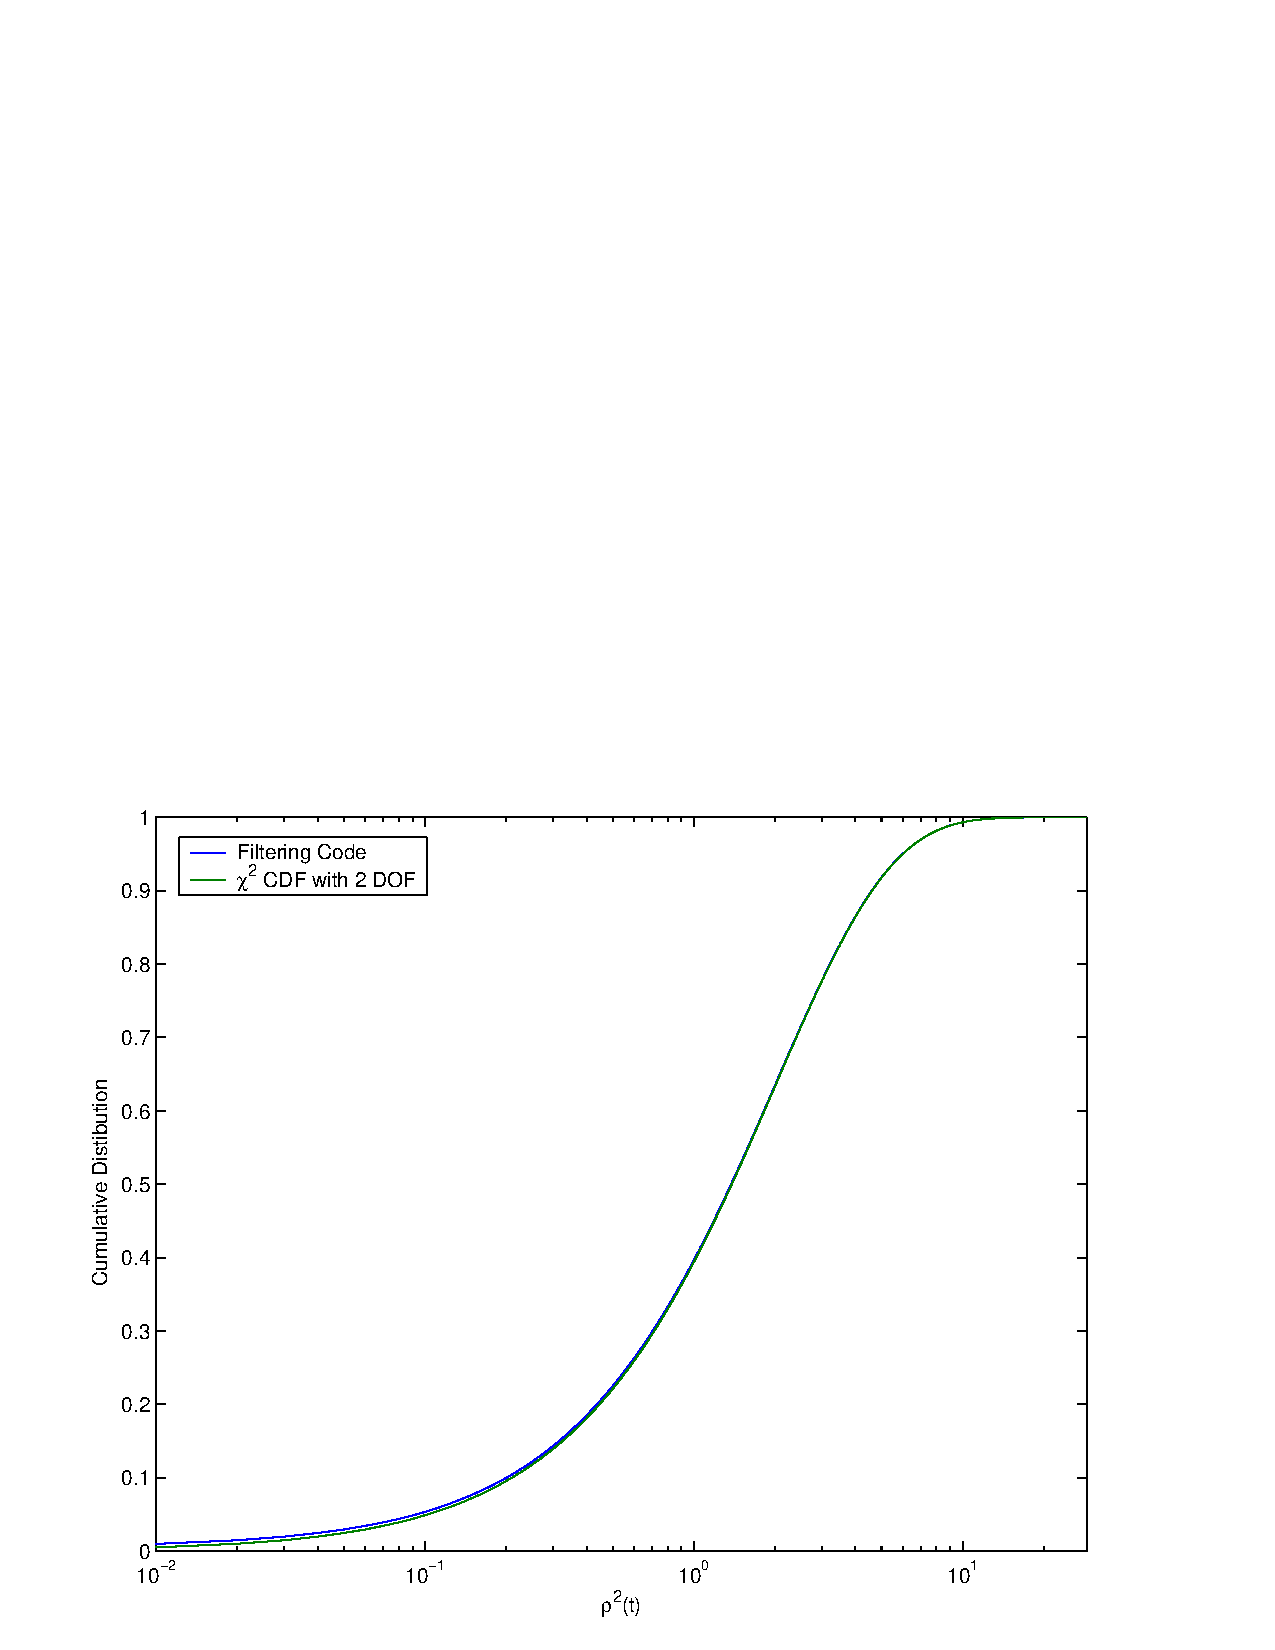
\includegraphics[width=\linewidth]{figures/findchirp/rhosq_gaussian_cdf}
\end{center}
\caption{%
In the presence of Gaussian noise the expected filter output, $\rho^2(t)$, is
the sum of the squares of two Gaussian distributed quantities and so should be
$\chi^2$ distributed with two degrees of freedom. This figure shows the
cumulative distribution function (CDF) of the filtering code output and the
expected analytic value. The filter input is white Gaussian noise of variance
$\nu$ and a constant power spectral density of $\ospsd = 2\nu^2\delta T$. It
can be seen that there is good agreement between the observed and expected
values.
}
\end{figure}

\begin{figure}[htb]
\label{f:impuse_snr}
\begin{center}
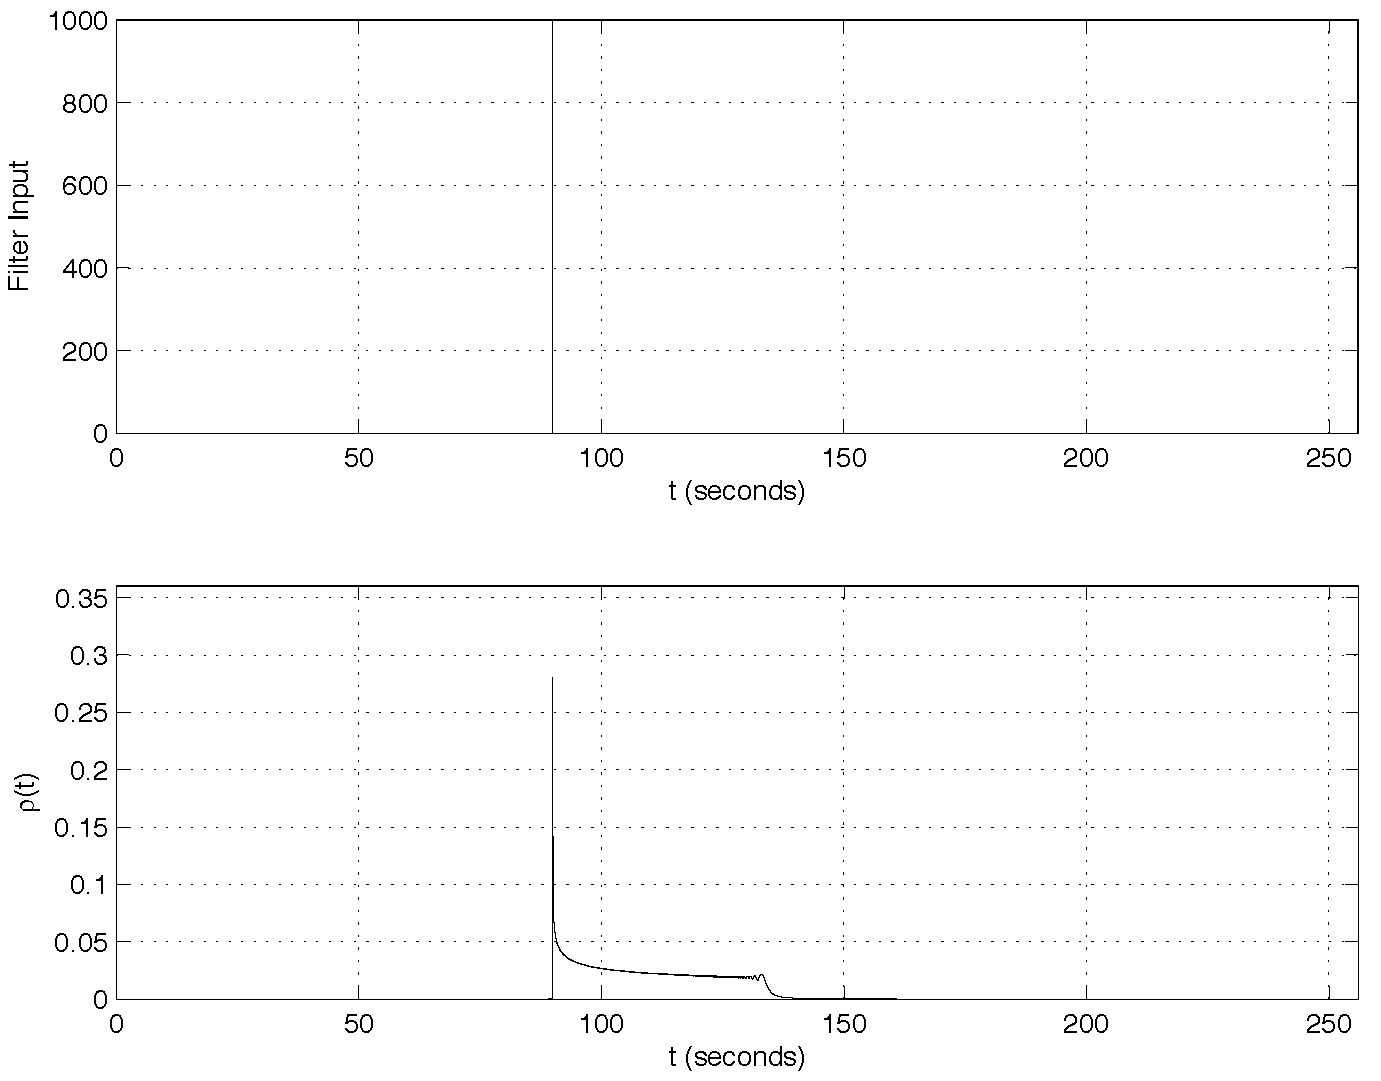
\includegraphics[width=\linewidth]{figures/findchirp/impulse_snr}
\end{center}
\caption{%
The top panel shows the filter input which consists of an impulse at $t_0 = 90$.
The power spectrum is set to that of white Gaussian noise. The bottom panel
shows the output of the filter. The filter output is the sum of the squares of
the time reverse chirps and the maximum of the filter output occurs at the
time of the impulse.
}
\end{figure}

\begin{figure}[htb]
\label{f:impuse_wraparound}
\begin{center}
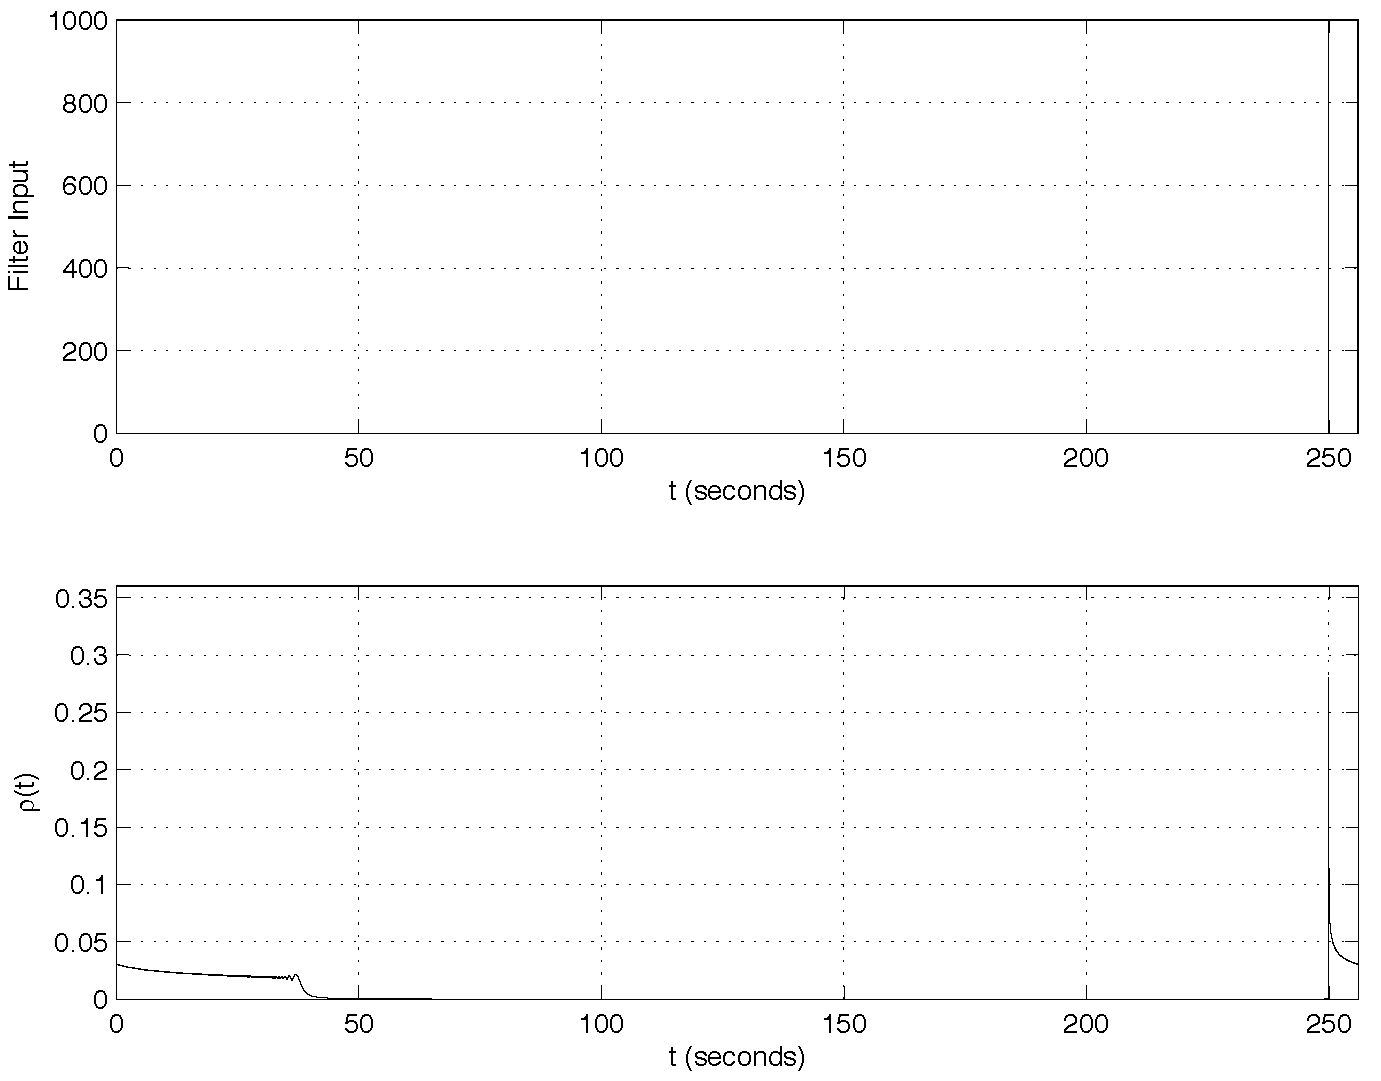
\includegraphics[width=\linewidth]{figures/findchirp/impulse_wraparound}
\end{center}
\caption{%
The top panel shows the filter input which consists of an impulse at $t_0 = 250$.
The power spectrum is set to that of white Gaussian noise. The bottom panel
shows the output of the filter. The length of the chirp template is $43.7$
seconds. Notice that the filter output is non-zero for the first $37.7$
seconds of the output due to the wrap-around of the FFT.
}
\end{figure}

\begin{figure}[htb]
\label{f:rhosq_median_cdf}
\begin{center}
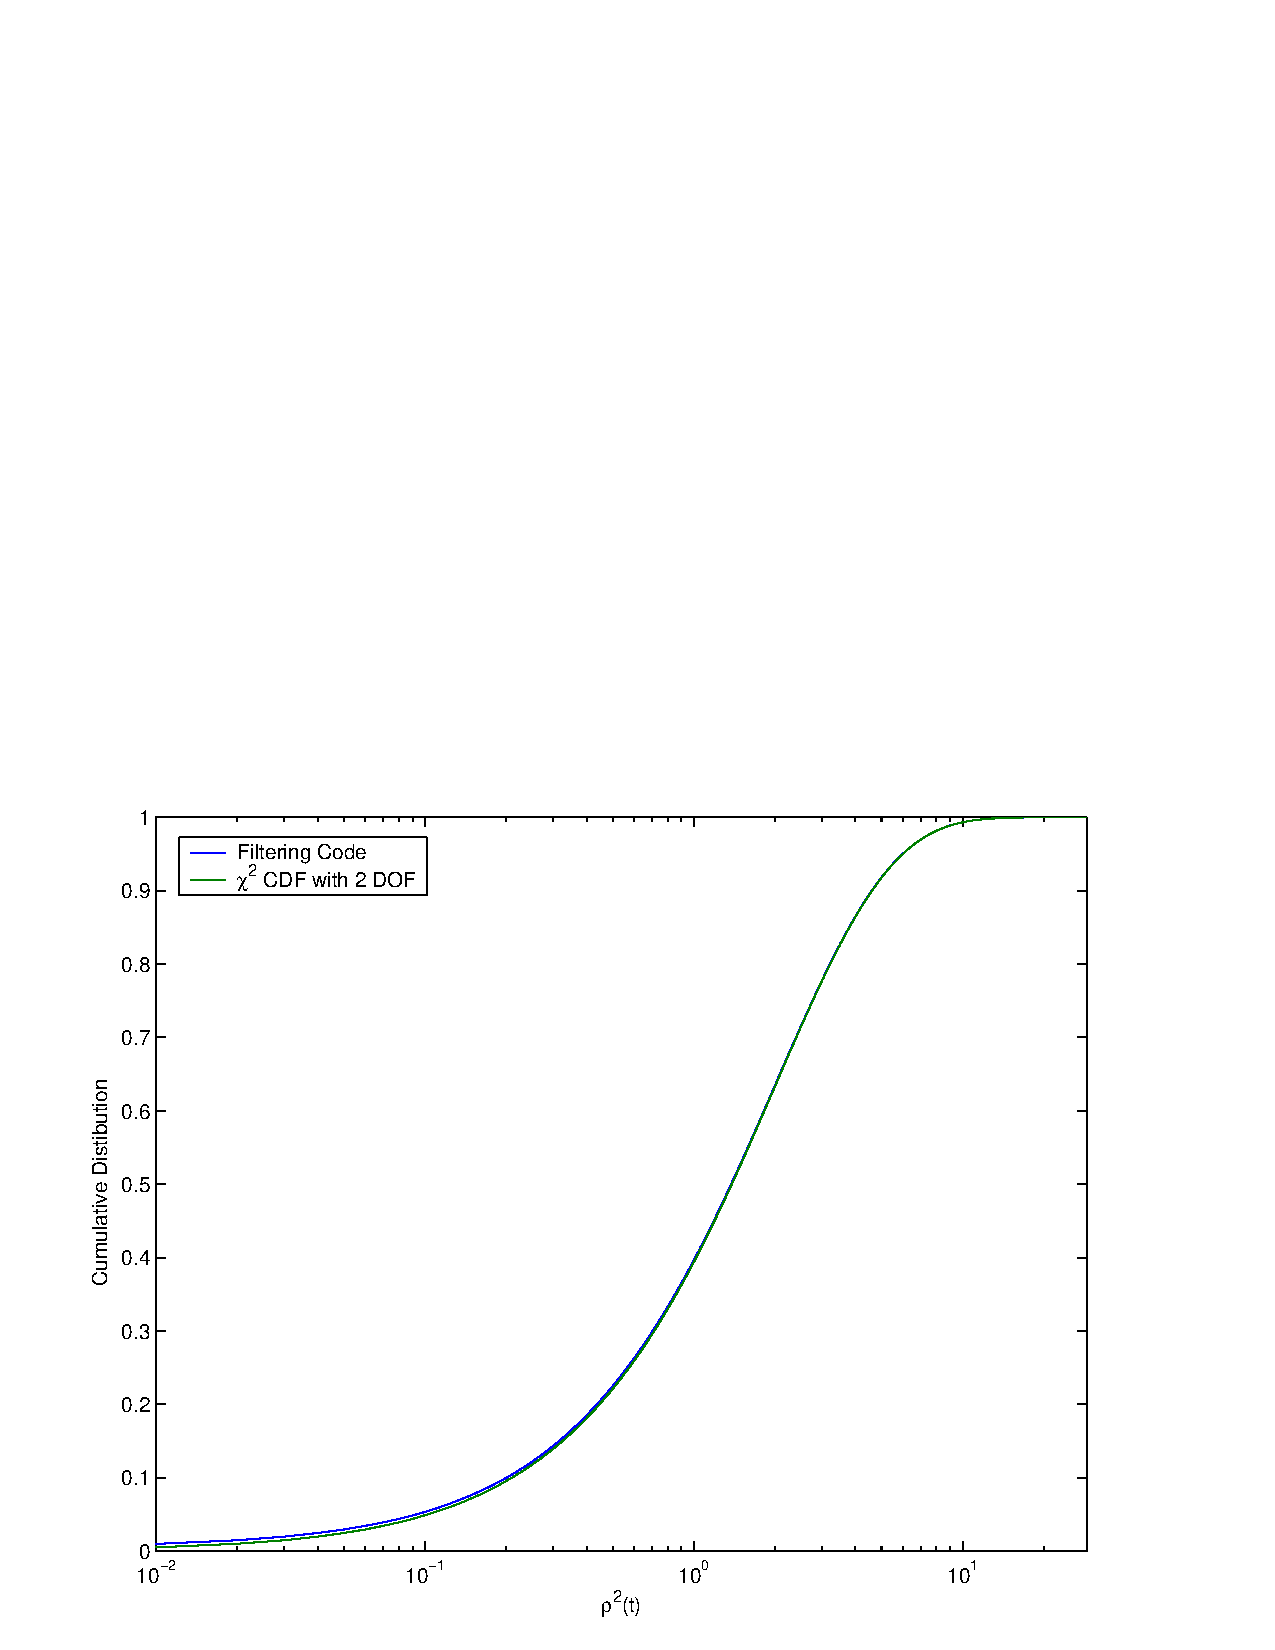
\includegraphics[width=\linewidth]{figures/findchirp/rhosq_gaussian_cdf}
\end{center}
\caption{%
In the presence of Gaussian noise the expected filter output, $\rho^2(t)$, is
the sum of the squares of two Gaussian distributed quantities and so should be
$\chi^2$ distributed with two degrees of freedom. This figure shows the
cumulative distribution function (CDF) of the filtering code output and the
expected analytic value. The filter input is white Gaussian noise of length
$256$ seconds and the power spectrum $\ospsd$ is computed from $15$ segments
of white Gaussian noise length $256$ seconds, overlapped by $128$ seconds
using Hann windowing and the median to estimator.
}
\end{figure}

\begin{figure}[htb]
\label{f:impulse_inv_spec}
\begin{center}
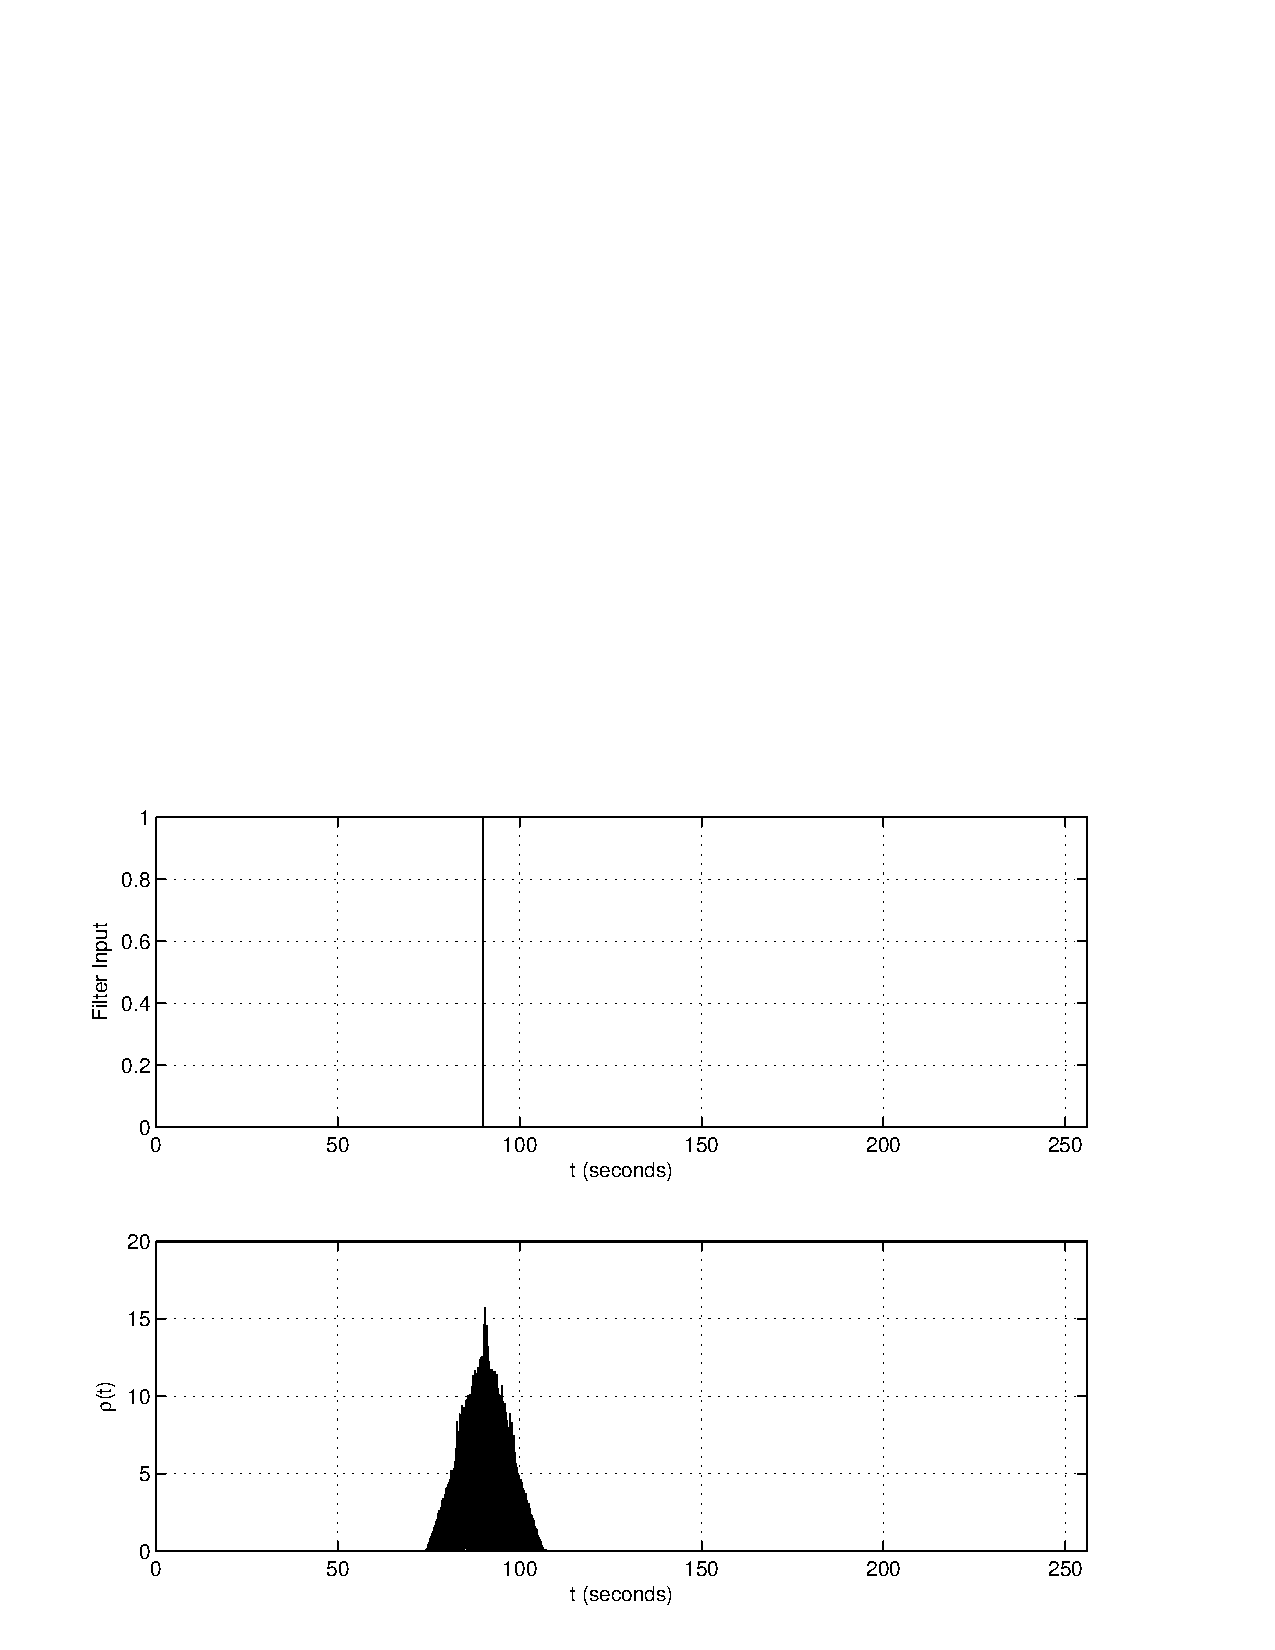
\includegraphics[width=\linewidth]{figures/findchirp/impulse_inv_spec}
\end{center}
\caption{%
The top panel shows the input to the filtering code which is an impulse at $t
= 90$ seconds. The average power spectrum is computed from typical LIGO noise
and then truncated to $16$ seconds in the time domain. The duration of non-zero
filter output is also $16$ seconds.
}
\end{figure}

\begin{figure}[htb]
\begin{center}
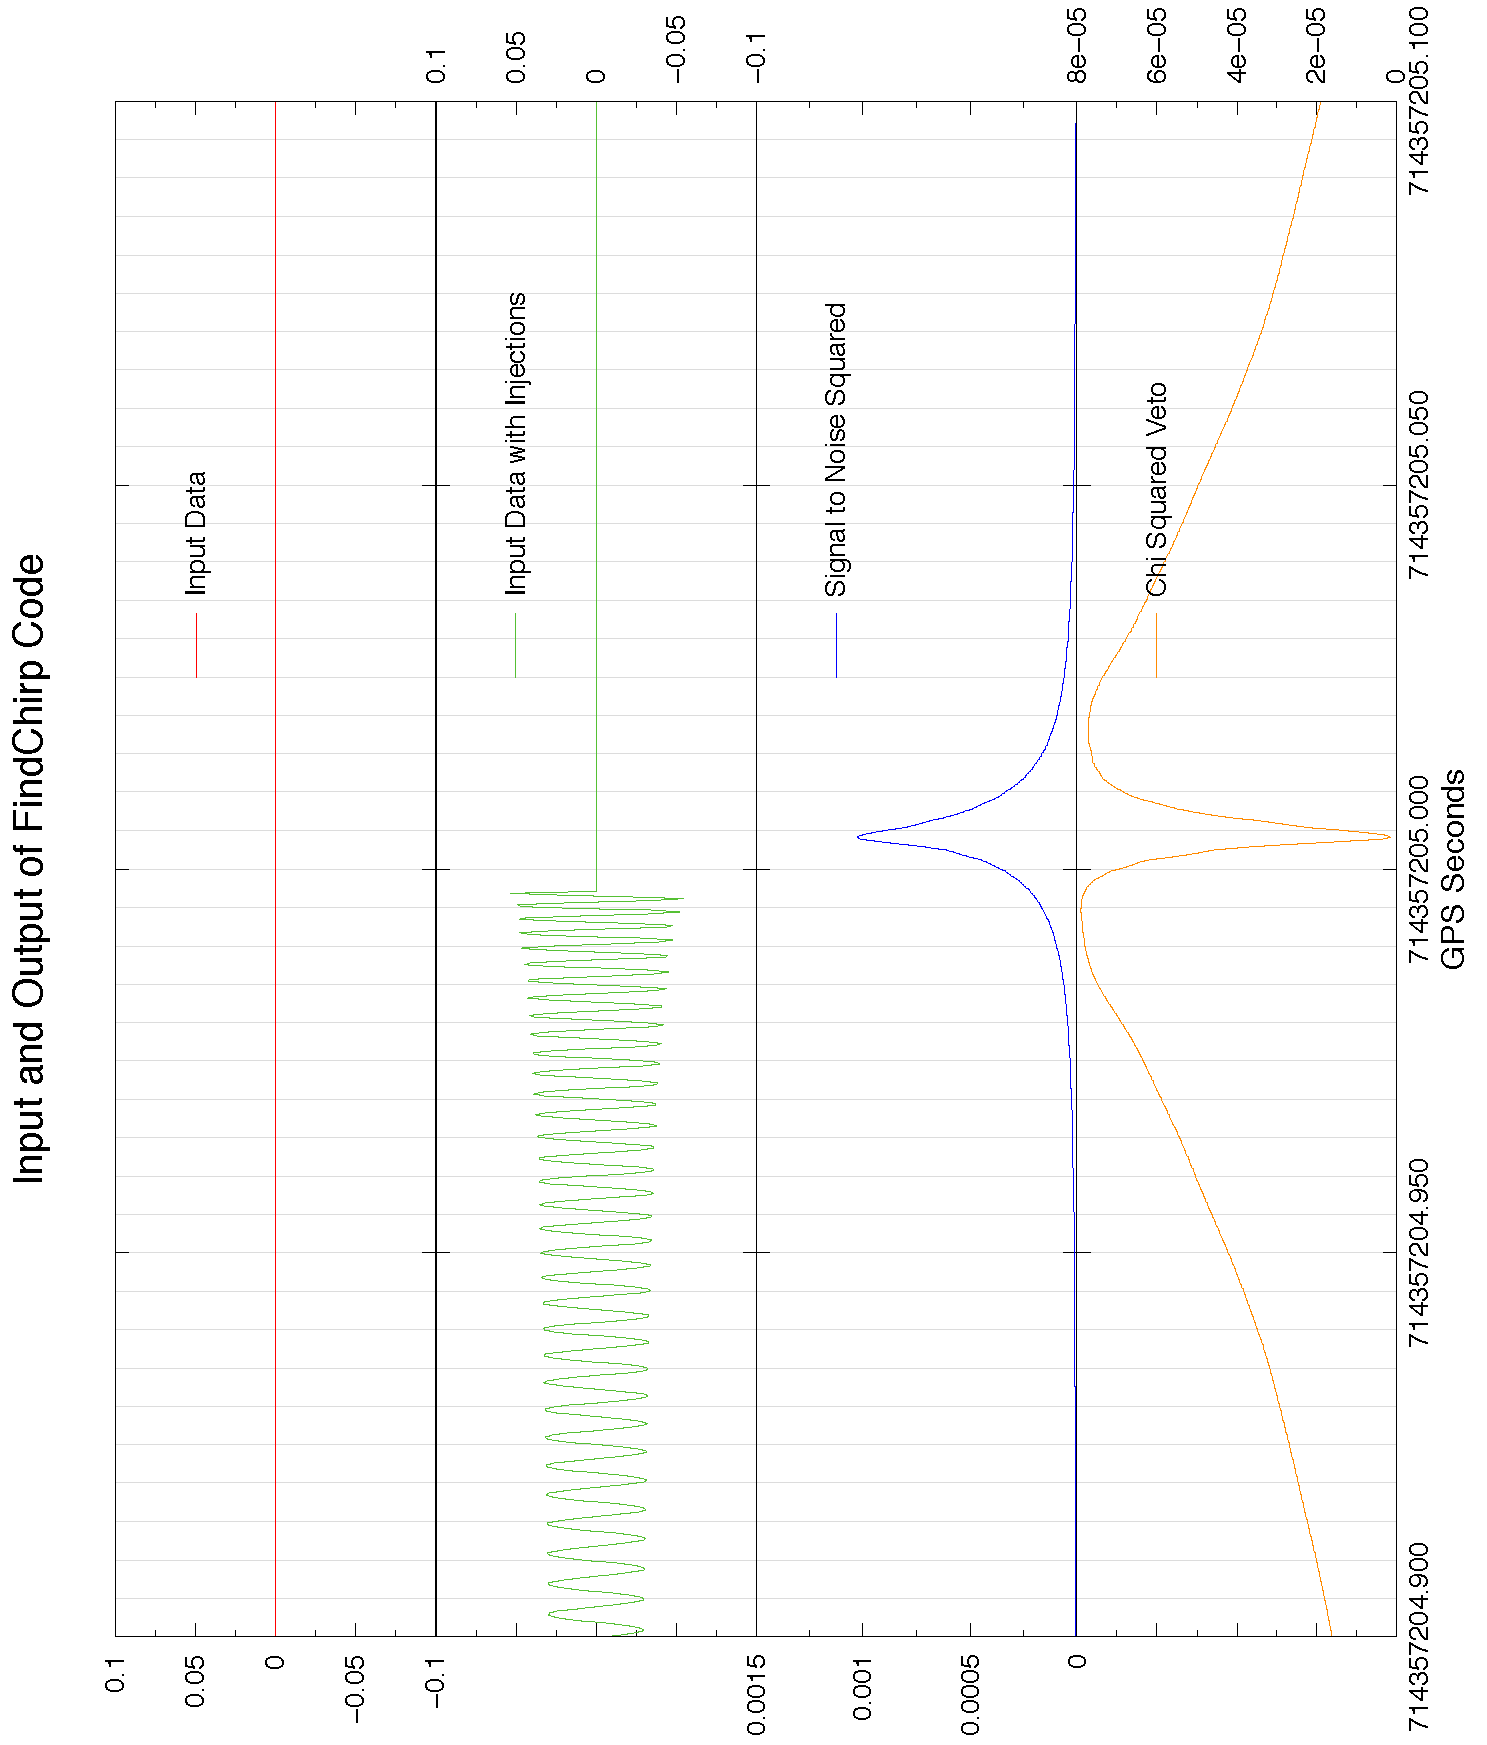
\includegraphics[angle=-90,width=0.75\linewidth]{figures/findchirp/zero_inject_zoom}
\end{center}
\caption{\label{f:zero_inject_zoom}Output time series from the filtering code
for an inspiral chirp in the absence of noise. A $(2.0,2.0)\,m_\odot$ inspiral
chirp is generated using the 2pN time domain waveform generation and injected
into the data. This is filtered using the 2pN stationary phase waveform. The
signal to noise squared and $\chi^2$ time series are shown.  The signal to
noise squared is a maximum at the coalescence time of the \textit{template}
inspiral signal. This occurs slightly after the coalescence time of the
injected signal. The difference in coalescence times is due to the different
methods of generating the chirp signal.
}
\end{figure}

